% !TEX program = xelatex
\documentclass[aspectratio=169,UTF8]{ctexbeamer}
\usetheme{Madrid}
\usecolortheme{default}

\usepackage{graphicx}
\usepackage{booktabs}
\usepackage{listings}
\usepackage{tikz}
\usepackage{multirow}

\title{Campus Bulletin Board System}
\subtitle{需求分析与项目计划}
\author{Group 10}
\institute{浙江大学}
\date{\today}

\begin{document}

\begin{frame}
    \titlepage
\end{frame}

\begin{frame}{目录}
    \tableofcontents
\end{frame}

% ============================================================
\section{需求分析}
% ============================================================

\begin{frame}{项目背景}
    \begin{block}{Background}
        \begin{itemize}
            \item \textbf{目标用户}：在校大学生、教职工、校园社团组织者。
            \item \textbf{项目目标}：构建一个功能完善、易于维护的校园论坛，支持话题分区、互动讨论与内容管理。
            \item \textbf{预期收益}：提升校园信息流通效率，形成可检索的知识库，支持社团活动宣传与学术交流。
        \end{itemize}
    \end{block}
\end{frame}

\begin{frame}{项目概述}
    \begin{block}{项目信息}
        \begin{itemize}
            \item \textbf{项目名称}：Campus Bulletin Board System（校园论坛）
            \item \textbf{项目描述}：面向大学校园的在线论坛系统
            \item \textbf{核心功能}：用户注册、发帖、评论、点赞、通知、搜索、管理后台
        \end{itemize}
    \end{block}
\end{frame}

\begin{frame}{功能性需求 —— 用户与认证}
    \begin{block}{需求描述}
        \begin{itemize}
            \item \textbf{UC-1 用户注册}：访客通过用户名/邮箱/密码注册账号，需校验唯一性。
            \item \textbf{UC-2 用户登录}：支持账号密码登录，成功后返回 JWT Token。
            \item \textbf{UC-3 密码重置}：已登录用户可修改密码，旧密码需校验。
            \item \textbf{UC-4 角色与权限}：区分普通用户与管理员，接口级权限控制。
        \end{itemize}
    \end{block}
\end{frame}

\begin{frame}{功能性需求 —— 帖子与分区}
    \begin{block}{需求描述}
        \begin{itemize}
            \item \textbf{UC-5 板块浏览}：按排序展示板块列表，支持查看板块下帖子。
            \item \textbf{UC-6 发帖}：登录用户在指定板块发布帖子，支持富文本/草稿。
            \item \textbf{UC-7 帖子管理}：作者可编辑/删除自己的帖子；管理员可置顶、加精、隐藏。
            \item \textbf{UC-8 列表查询}：支持分页、排序（最新/最热），返回帖子摘要。
        \end{itemize}
    \end{block}
\end{frame}

\begin{frame}{功能性需求 —— 评论、互动与通知}
    \begin{columns}
        \column{0.48\textwidth}
        \begin{block}{评论与互动}
            \begin{itemize}
                \item \textbf{UC-9} 评论发布与回复（楼中楼）
                \item \textbf{UC-10} 点赞/取消点赞（帖子、评论）
                \item \textbf{UC-11} 实时计数聚合（点赞数、评论数）
            \end{itemize}
        \end{block}
        \column{0.48\textwidth}
        \begin{block}{通知与消息}
            \begin{itemize}
                \item \textbf{UC-12} 评论/回复/点赞触发通知
                \item \textbf{UC-13} 未读计数与已读标记
                \item \textbf{UC-14} 系统公告与站内信
            \end{itemize}
        \end{block}
    \end{columns}
\end{frame}

\begin{frame}{功能性需求 —— 管理后台}
    \begin{block}{需求描述}
        \begin{itemize}
            \item \textbf{UC-15 用户管理}：管理员可查看用户列表、封禁/解封、调整角色。
            \item \textbf{UC-16 板块/公告管理}：CRUD 板块，发布/编辑/下架系统公告。
            \item \textbf{UC-17 内容审核}：对帖子/评论进行隐藏/恢复/删除（软删除）。
            \item \textbf{UC-18 举报处理}：查看举报列表，处理并记录。
        \end{itemize}
    \end{block}
\end{frame}

\begin{frame}{用例图}
    \centering
    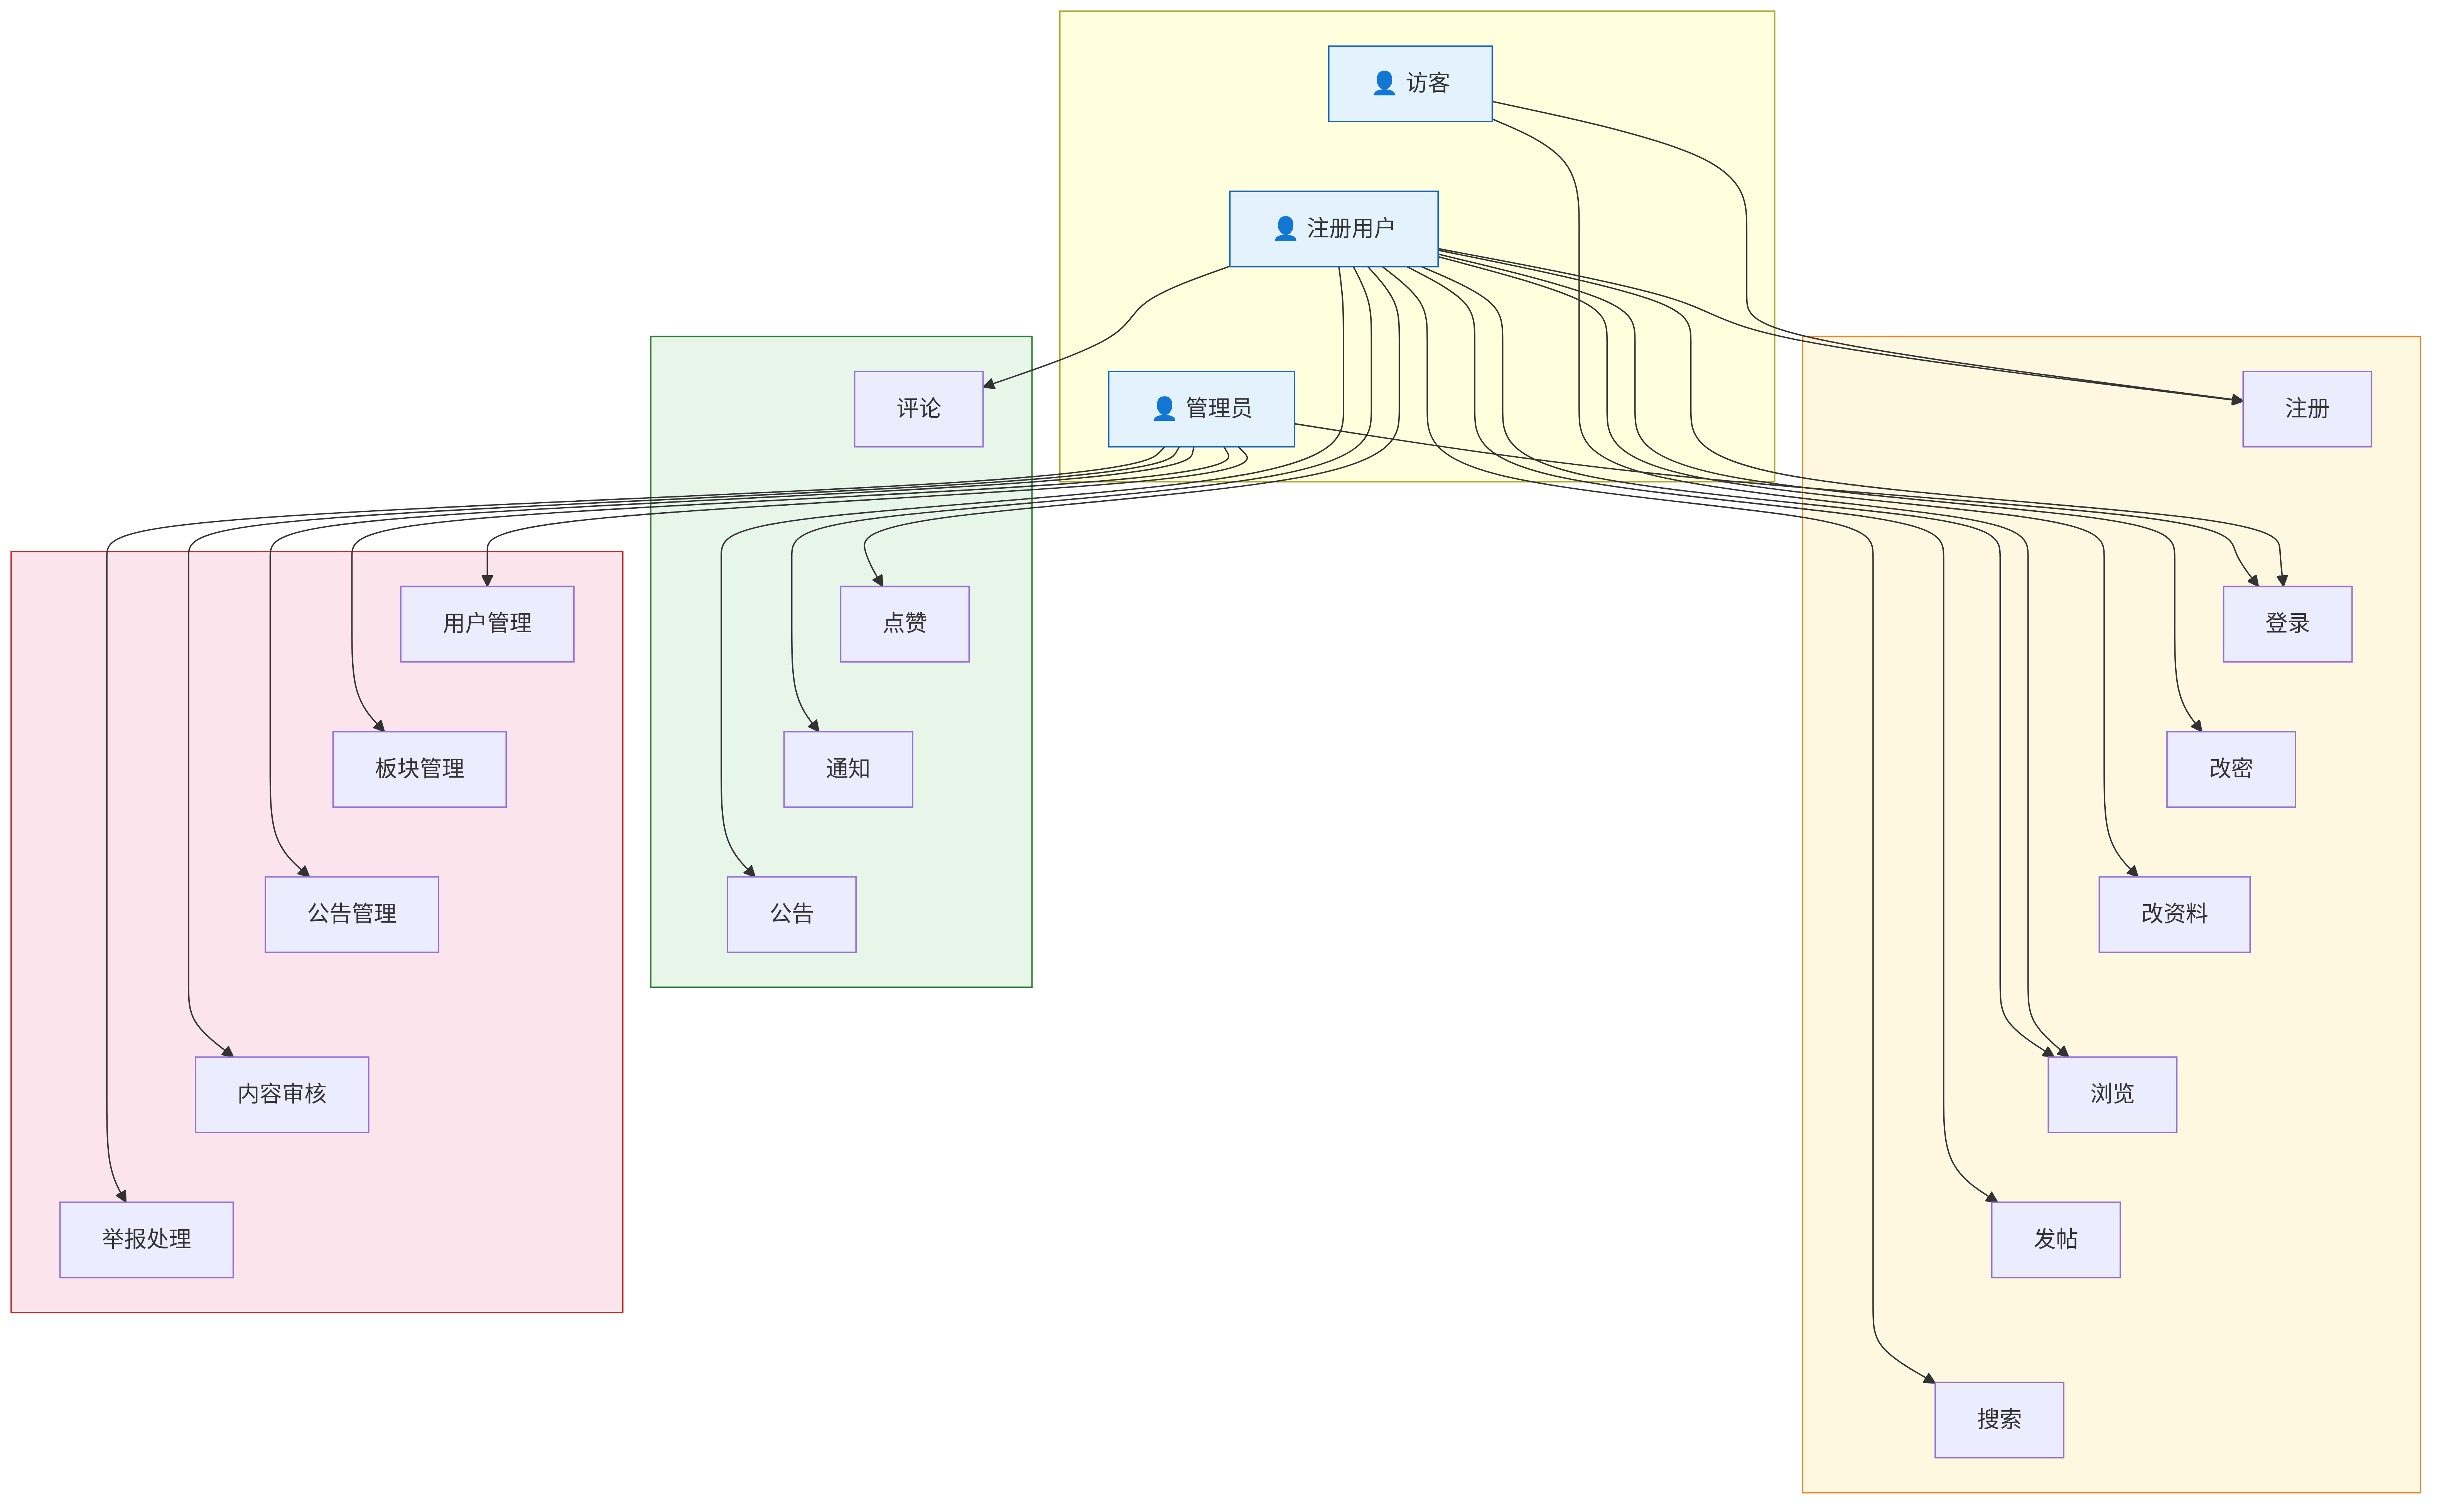
\includegraphics[width=\linewidth,height=0.88\textheight,keepaspectratio]{images/usecase_diagram.png}
\end{frame}

\begin{frame}{系统上下文数据流图}
    \centering
    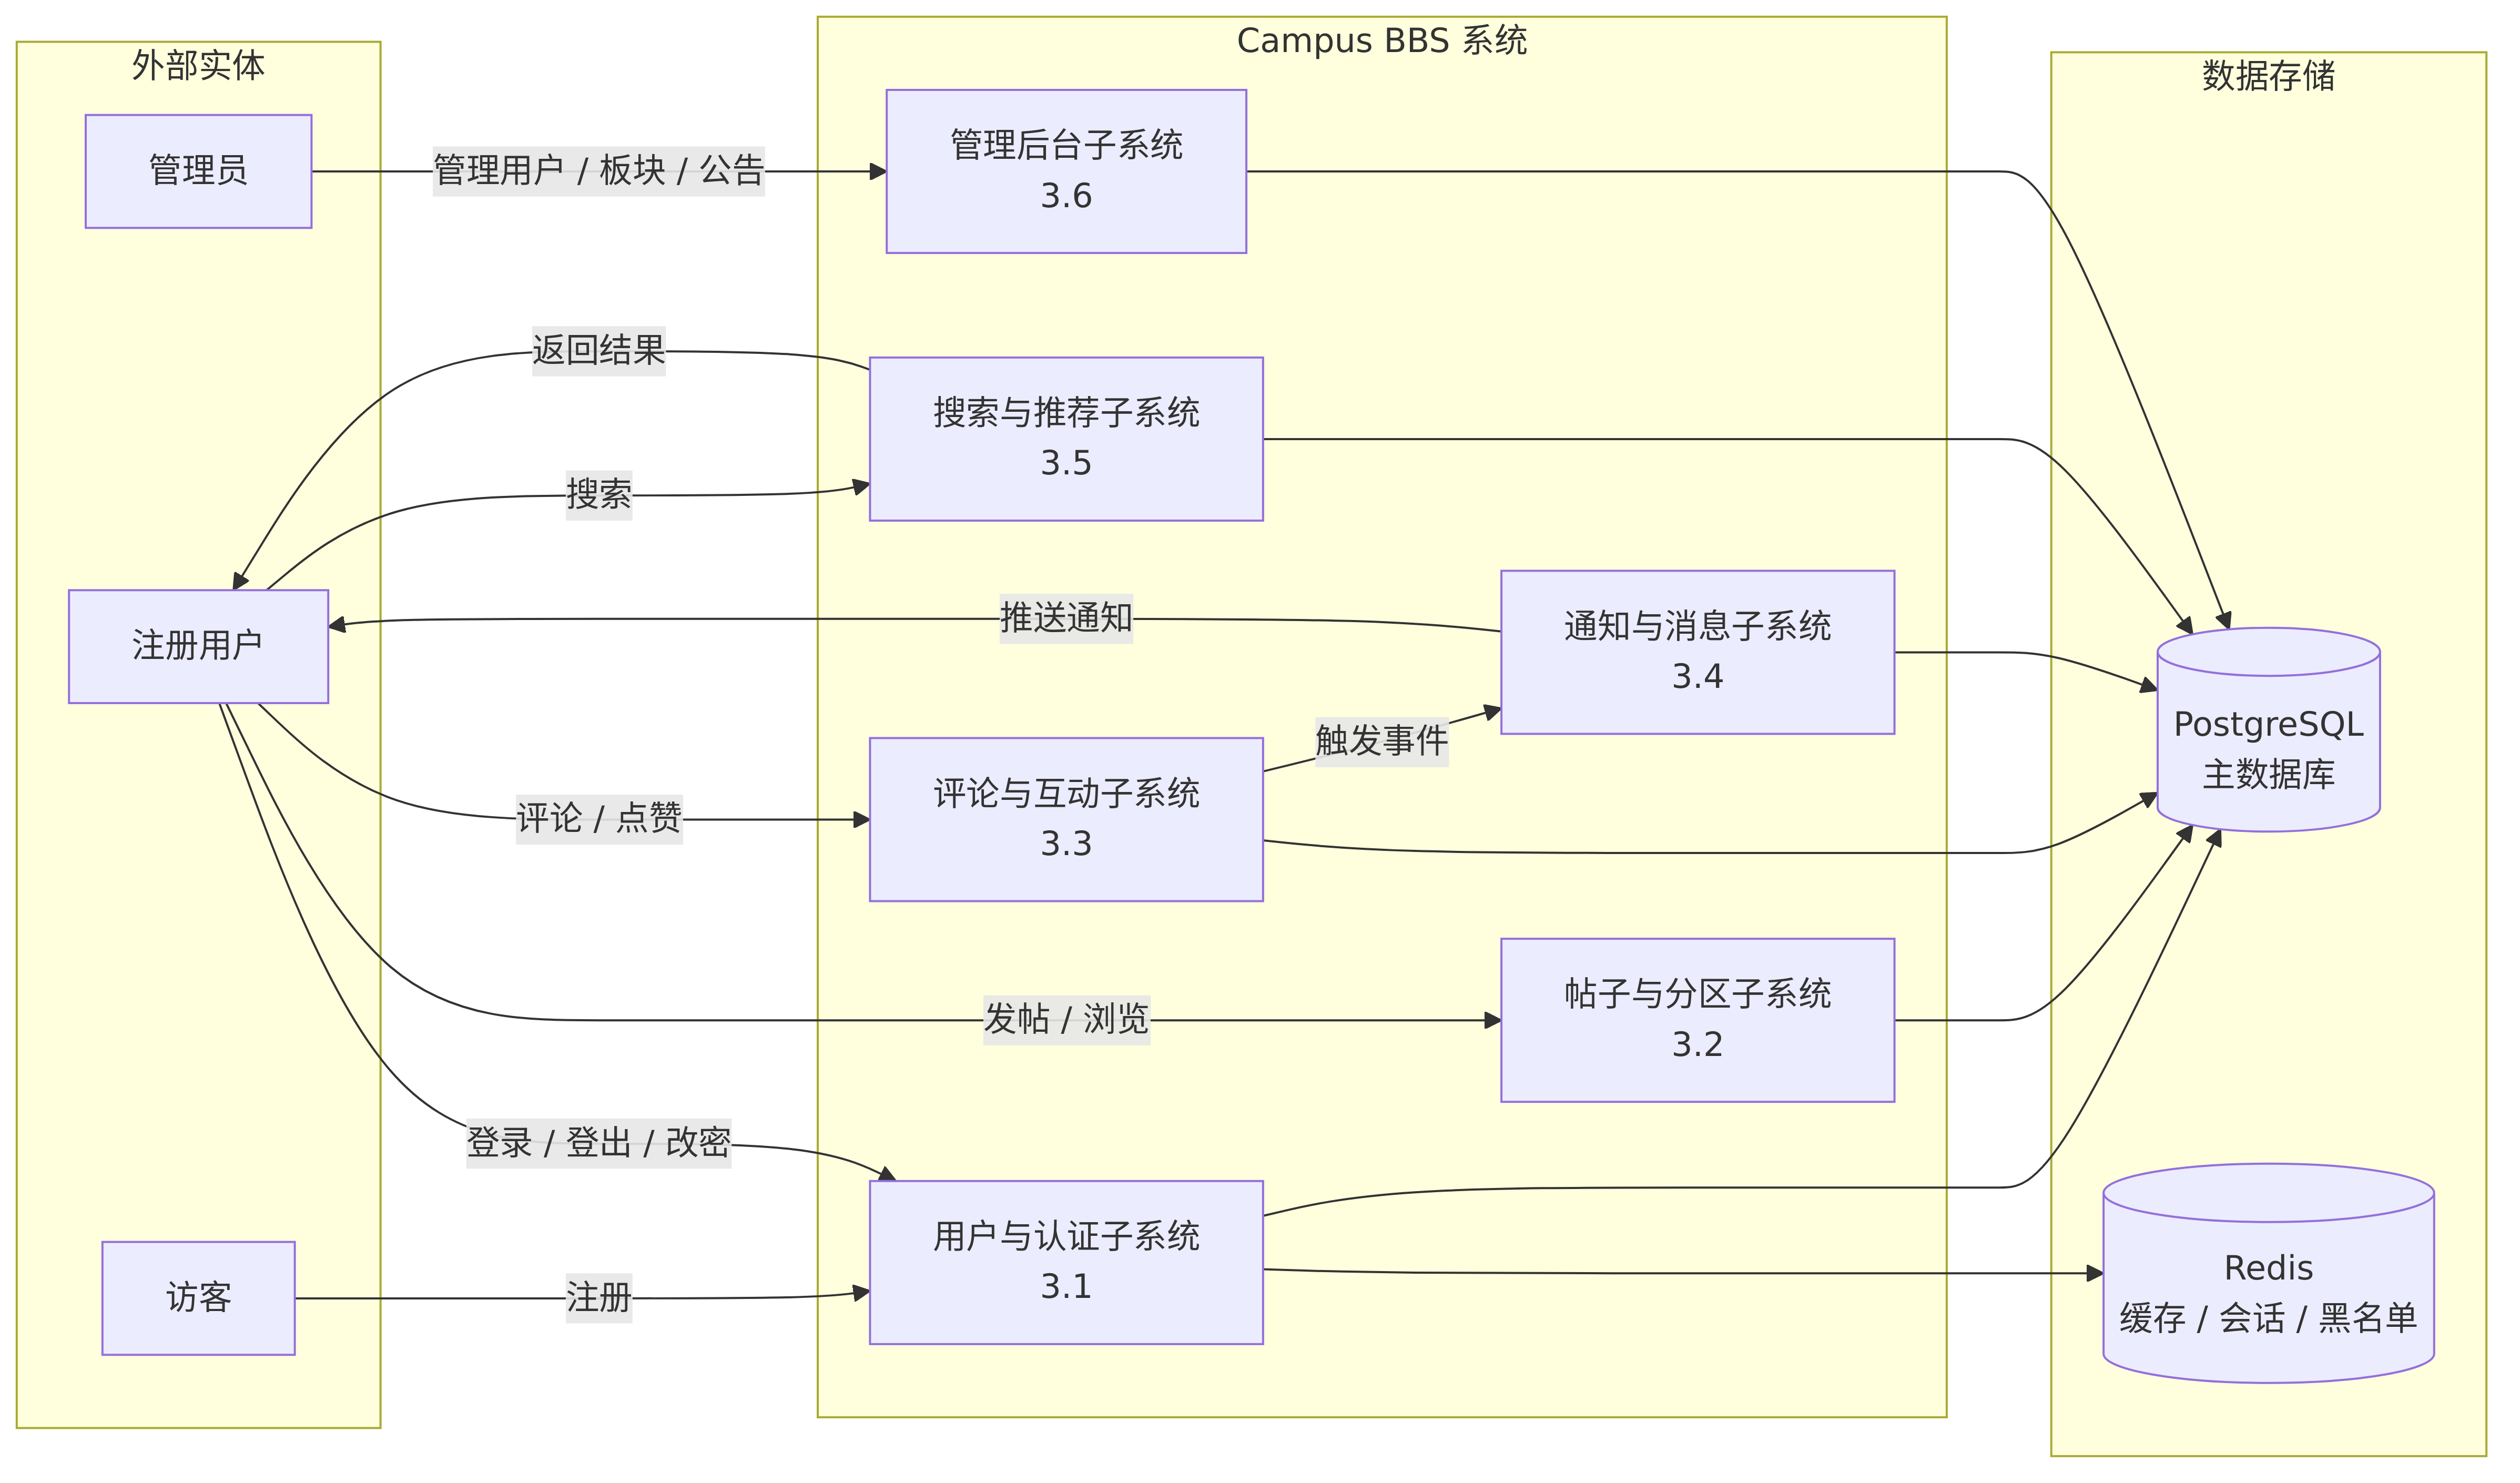
\includegraphics[width=\linewidth,height=0.88\textheight,keepaspectratio]{images/context_dfd.png}
\end{frame}

\begin{frame}{第0层数据流图}
    \centering
    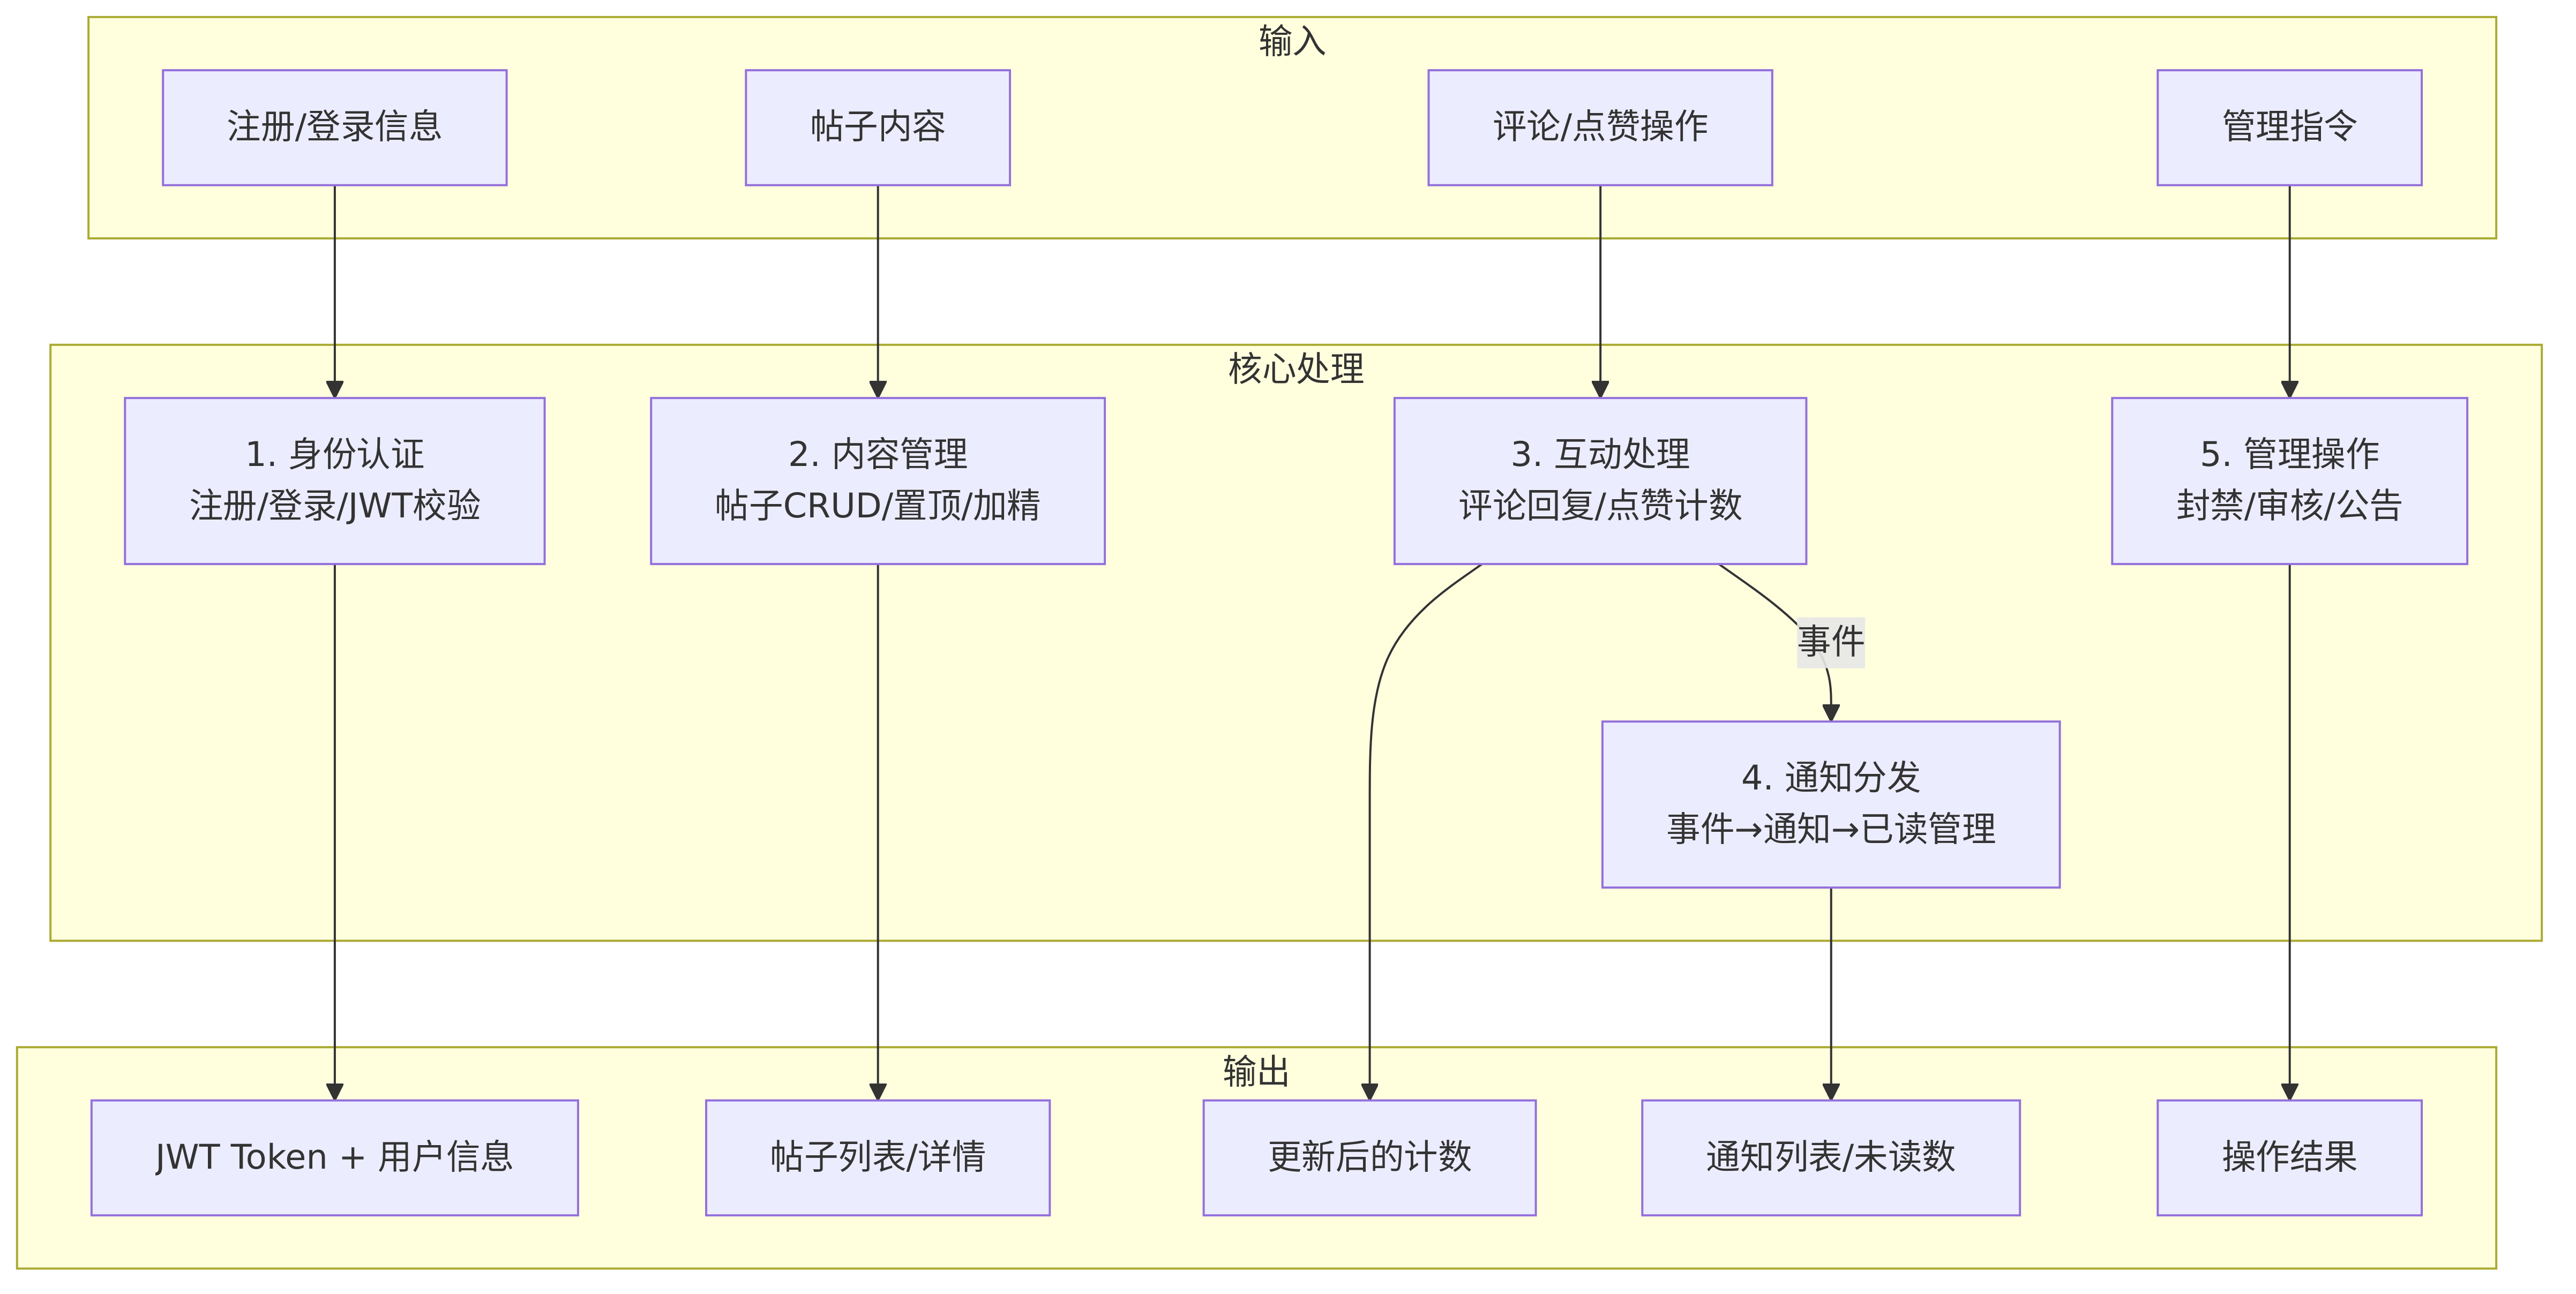
\includegraphics[width=\linewidth,height=0.88\textheight,keepaspectratio]{images/level0_dfd.png}
\end{frame}

\begin{frame}{状态图 —— 用户生命周期}
    \centering
    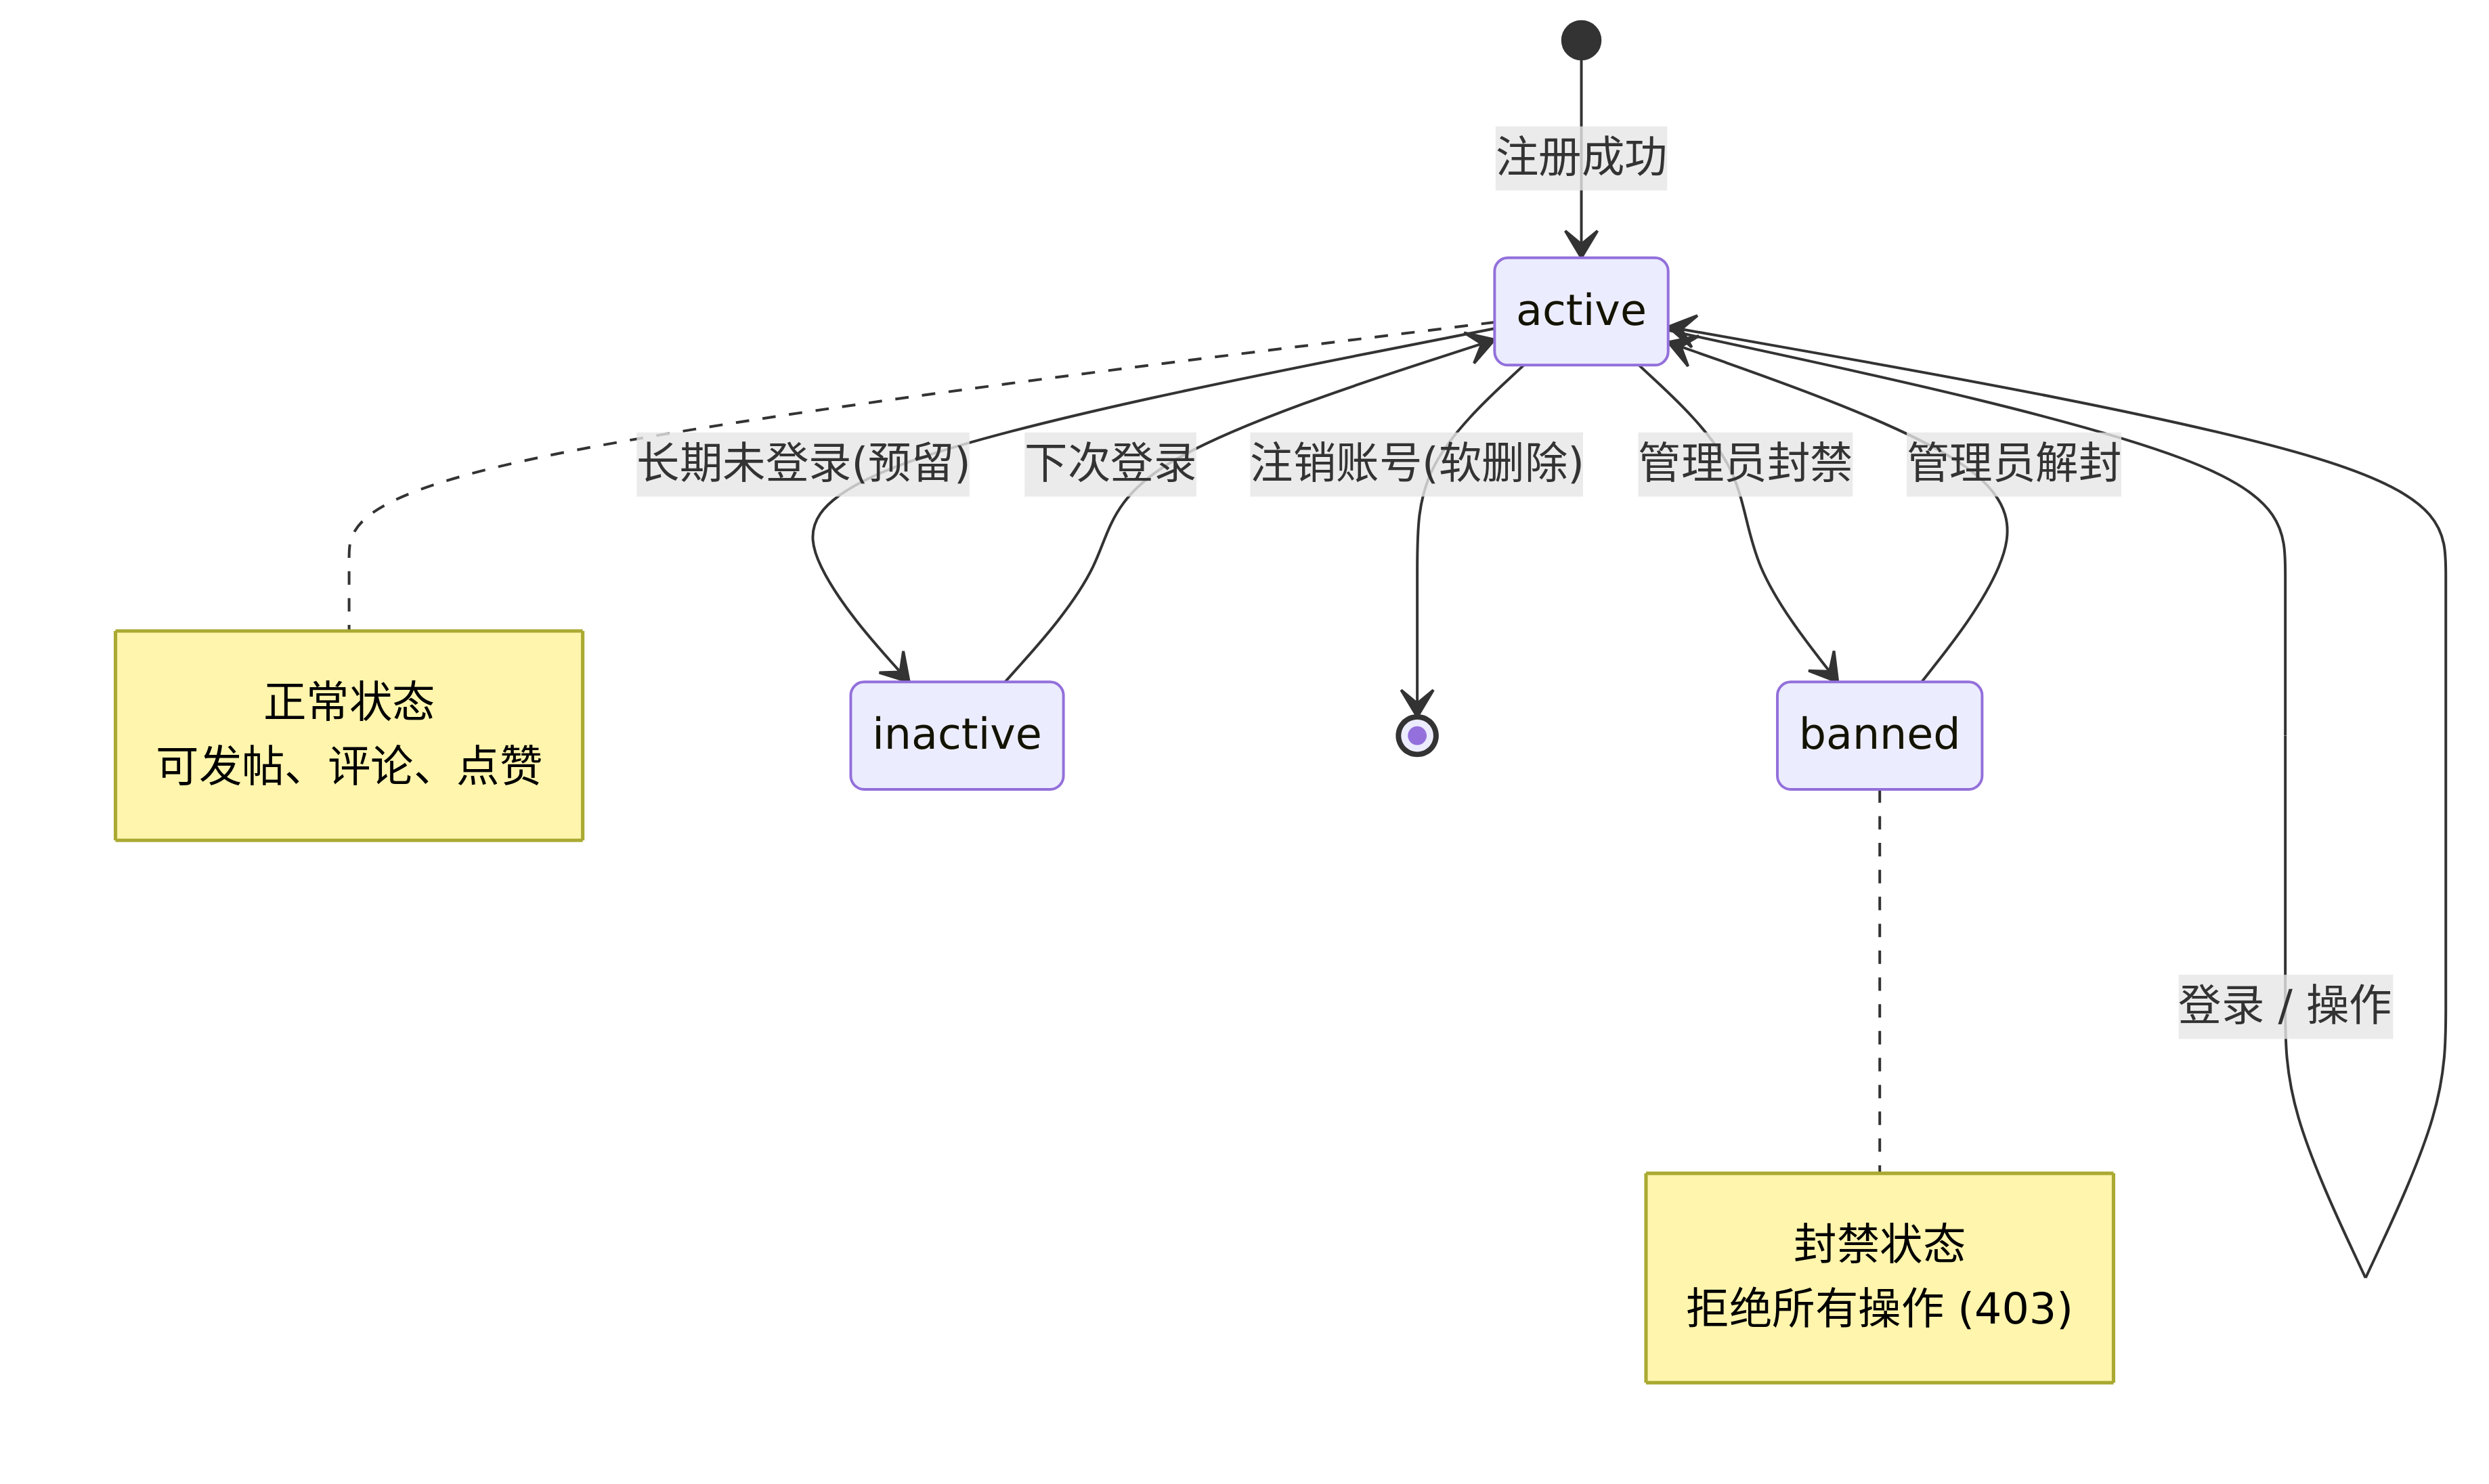
\includegraphics[width=\linewidth,height=0.88\textheight,keepaspectratio]{images/user_state.png}
\end{frame}

\begin{frame}{状态图 —— 帖子与评论}
    \centering
    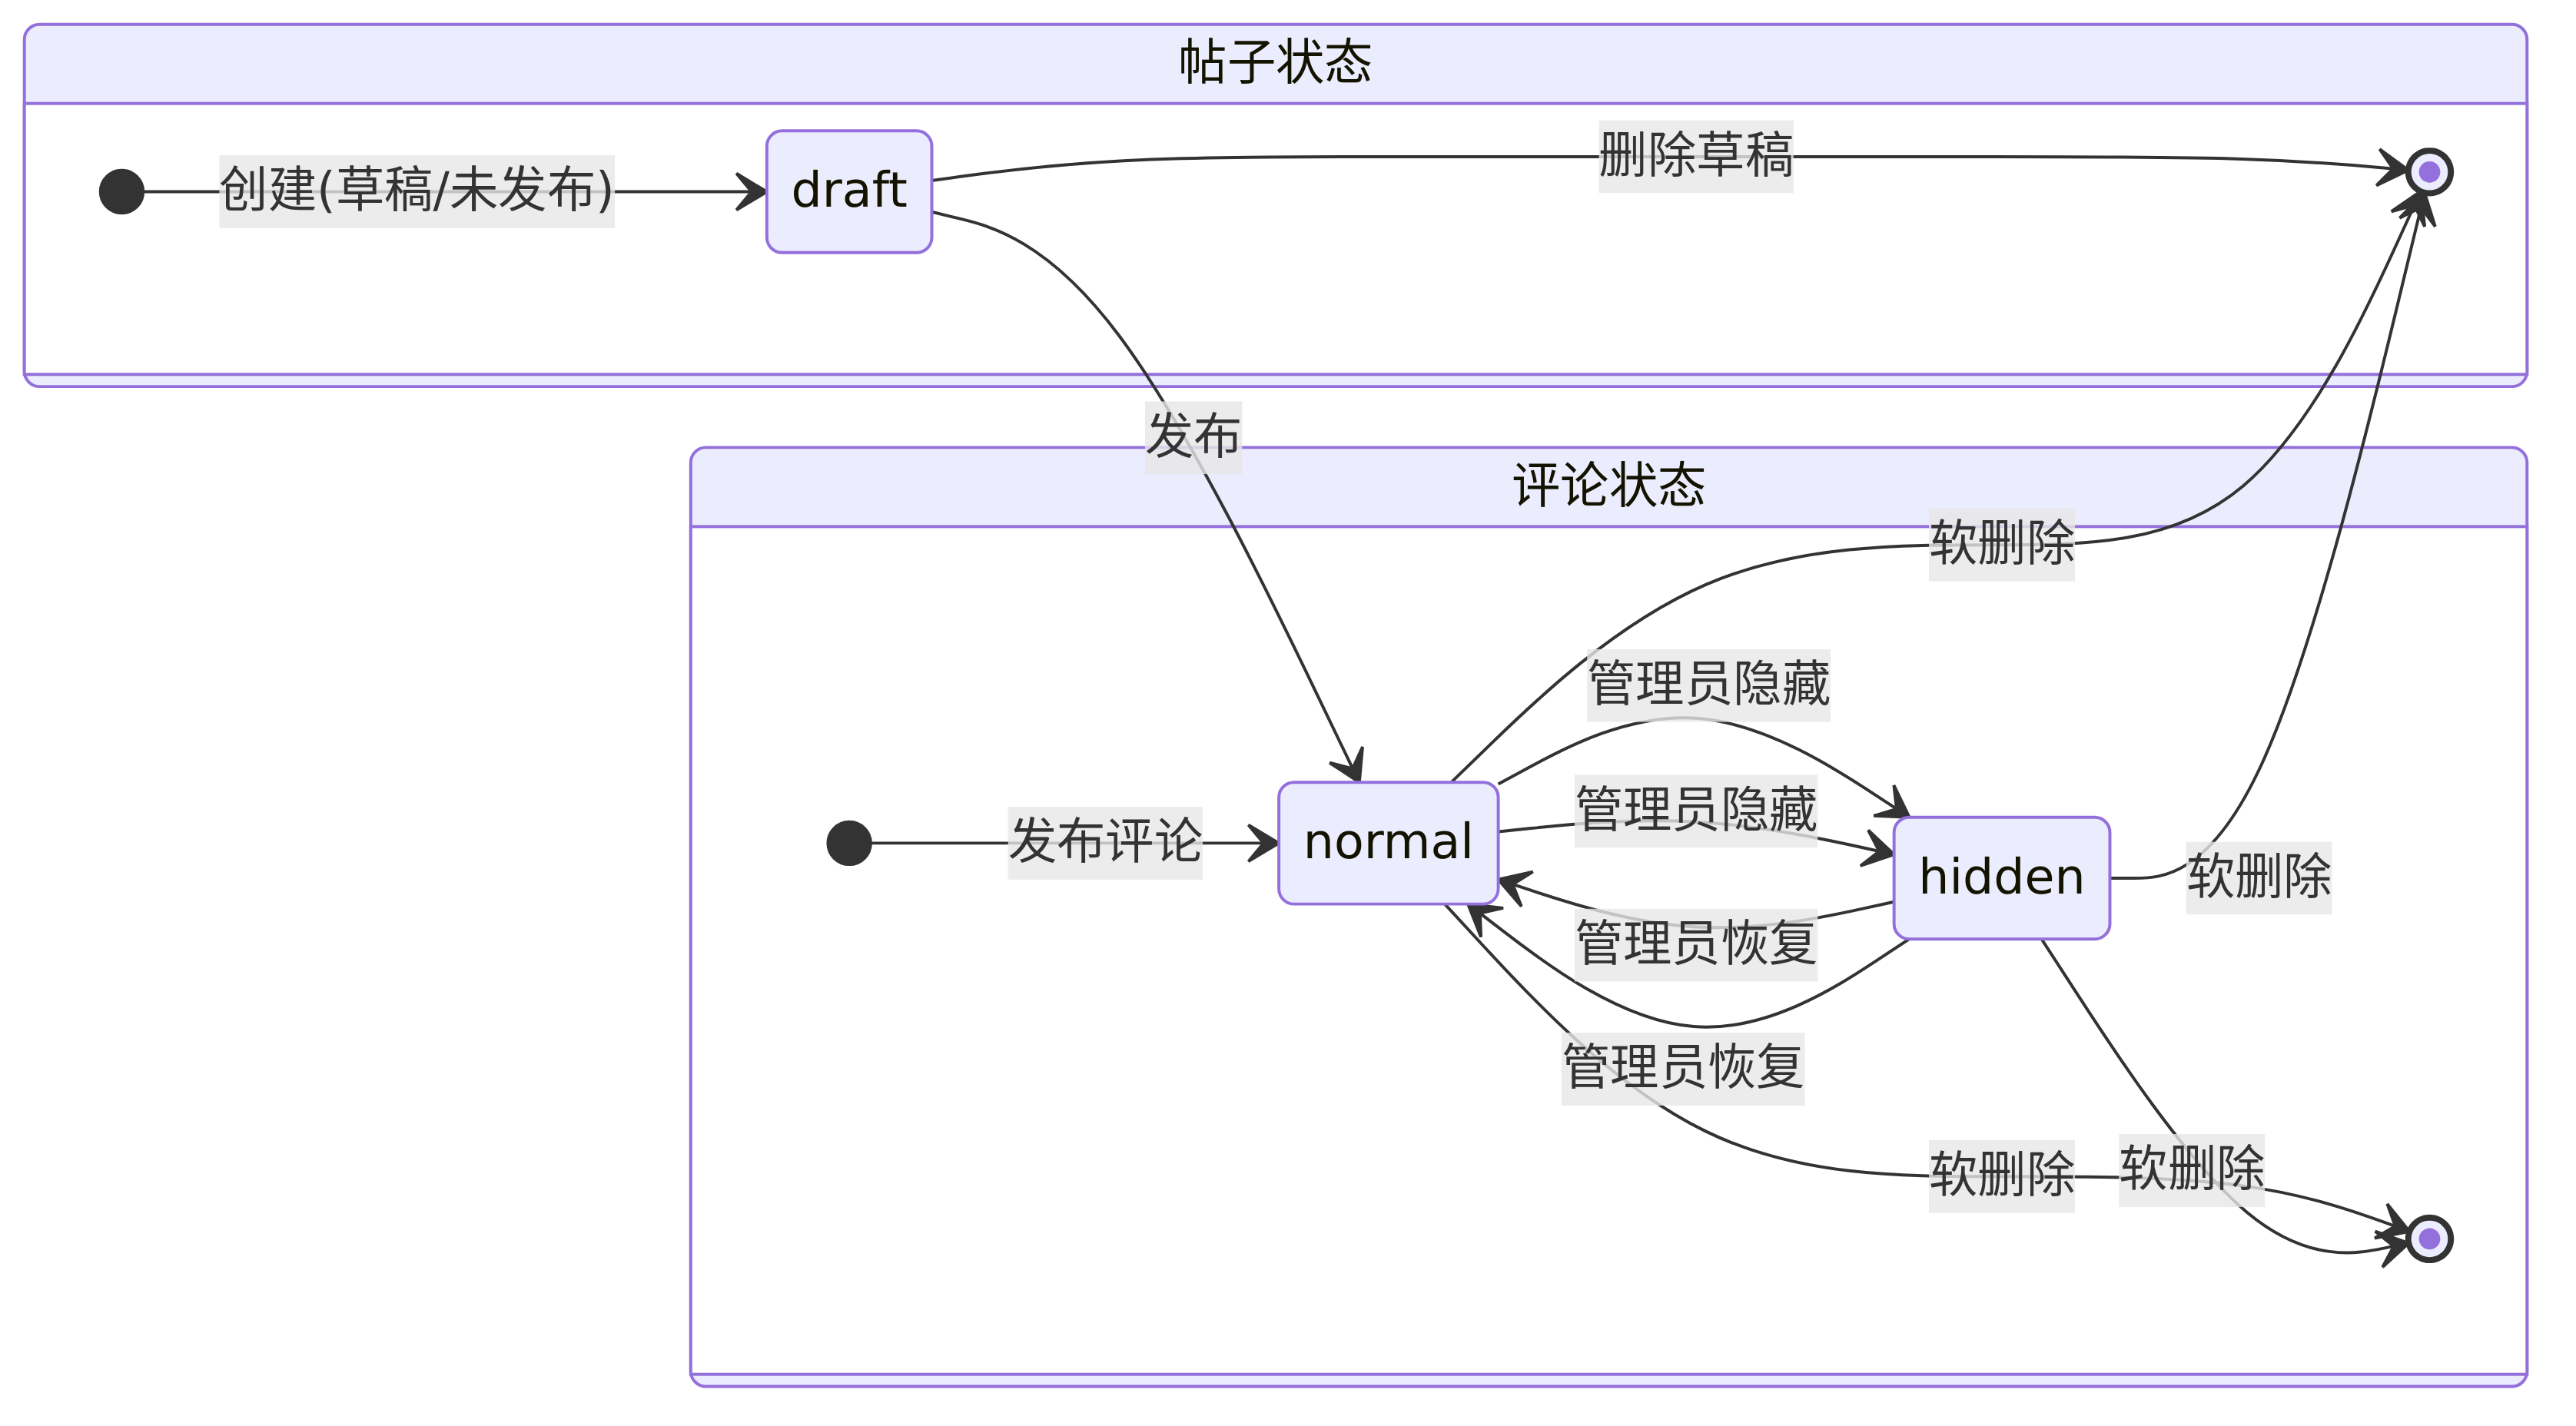
\includegraphics[width=\linewidth,height=0.88\textheight,keepaspectratio]{images/post_comment_state.png}
\end{frame}

\begin{frame}{状态图 —— 通知生命周期}
    \centering
    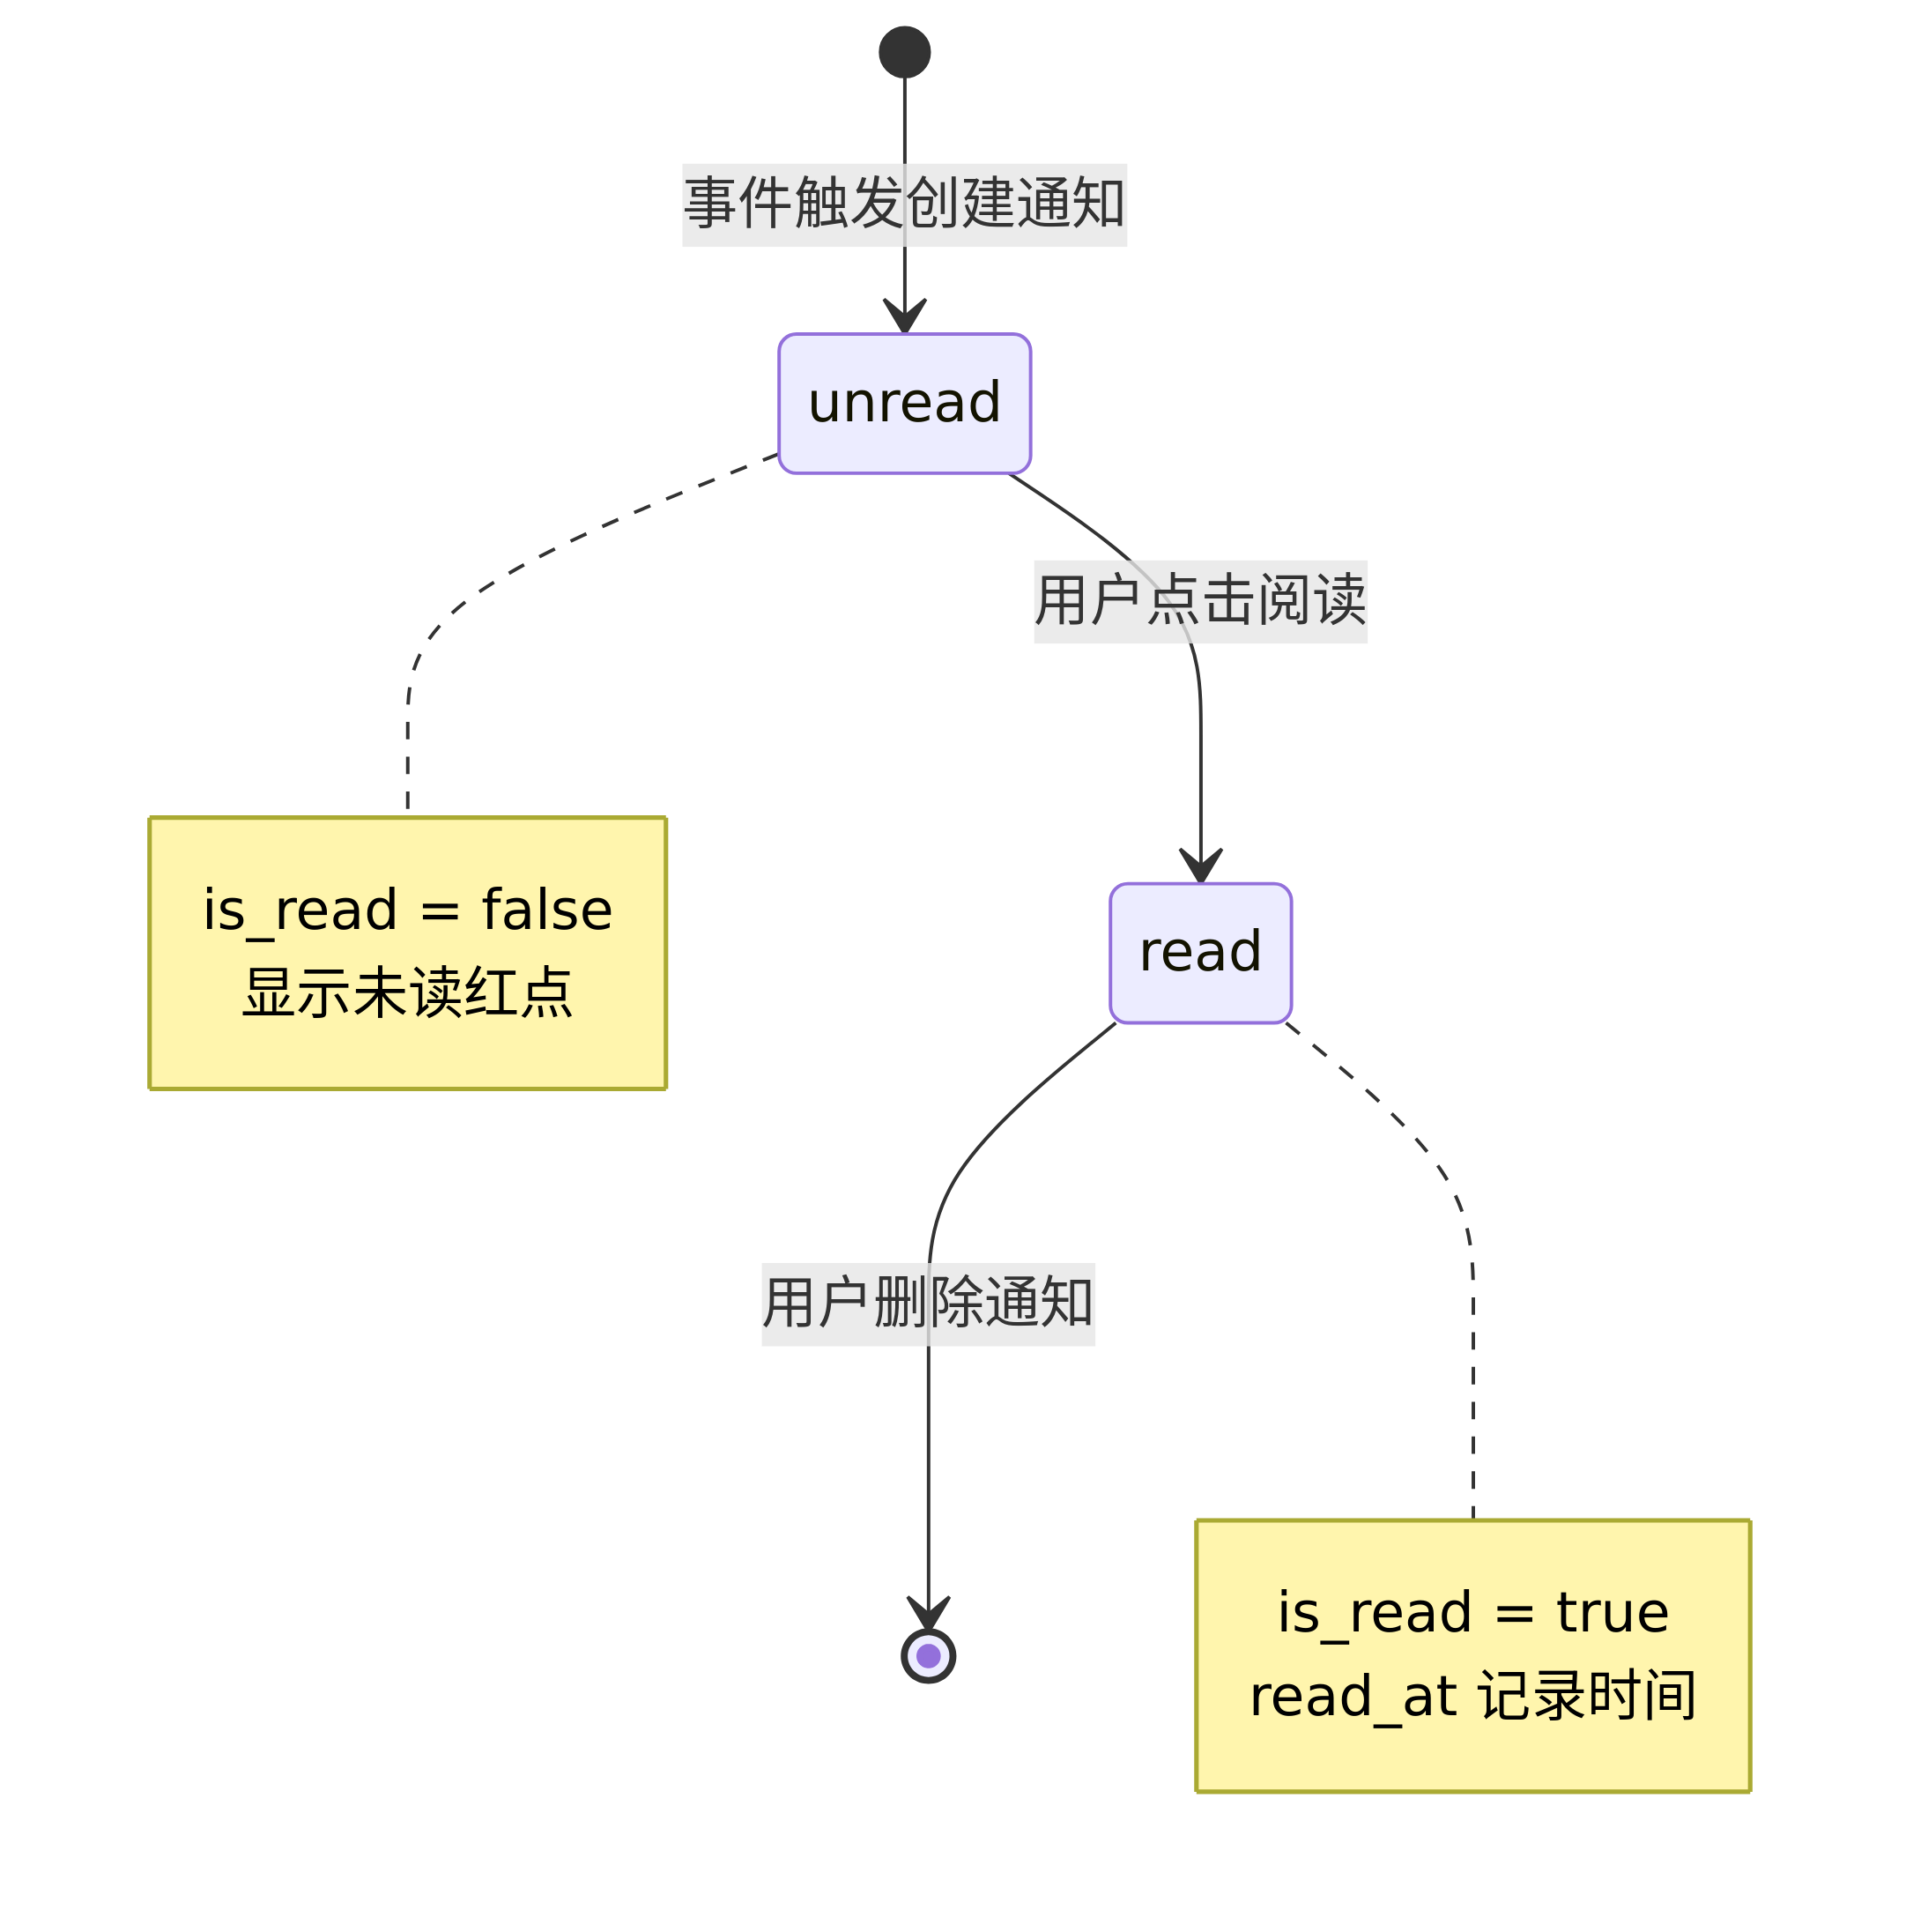
\includegraphics[width=\linewidth,height=0.88\textheight,keepaspectratio]{images/notification_state.png}
\end{frame}

\begin{frame}{类图 —— 后端核心模型}
    \centering
    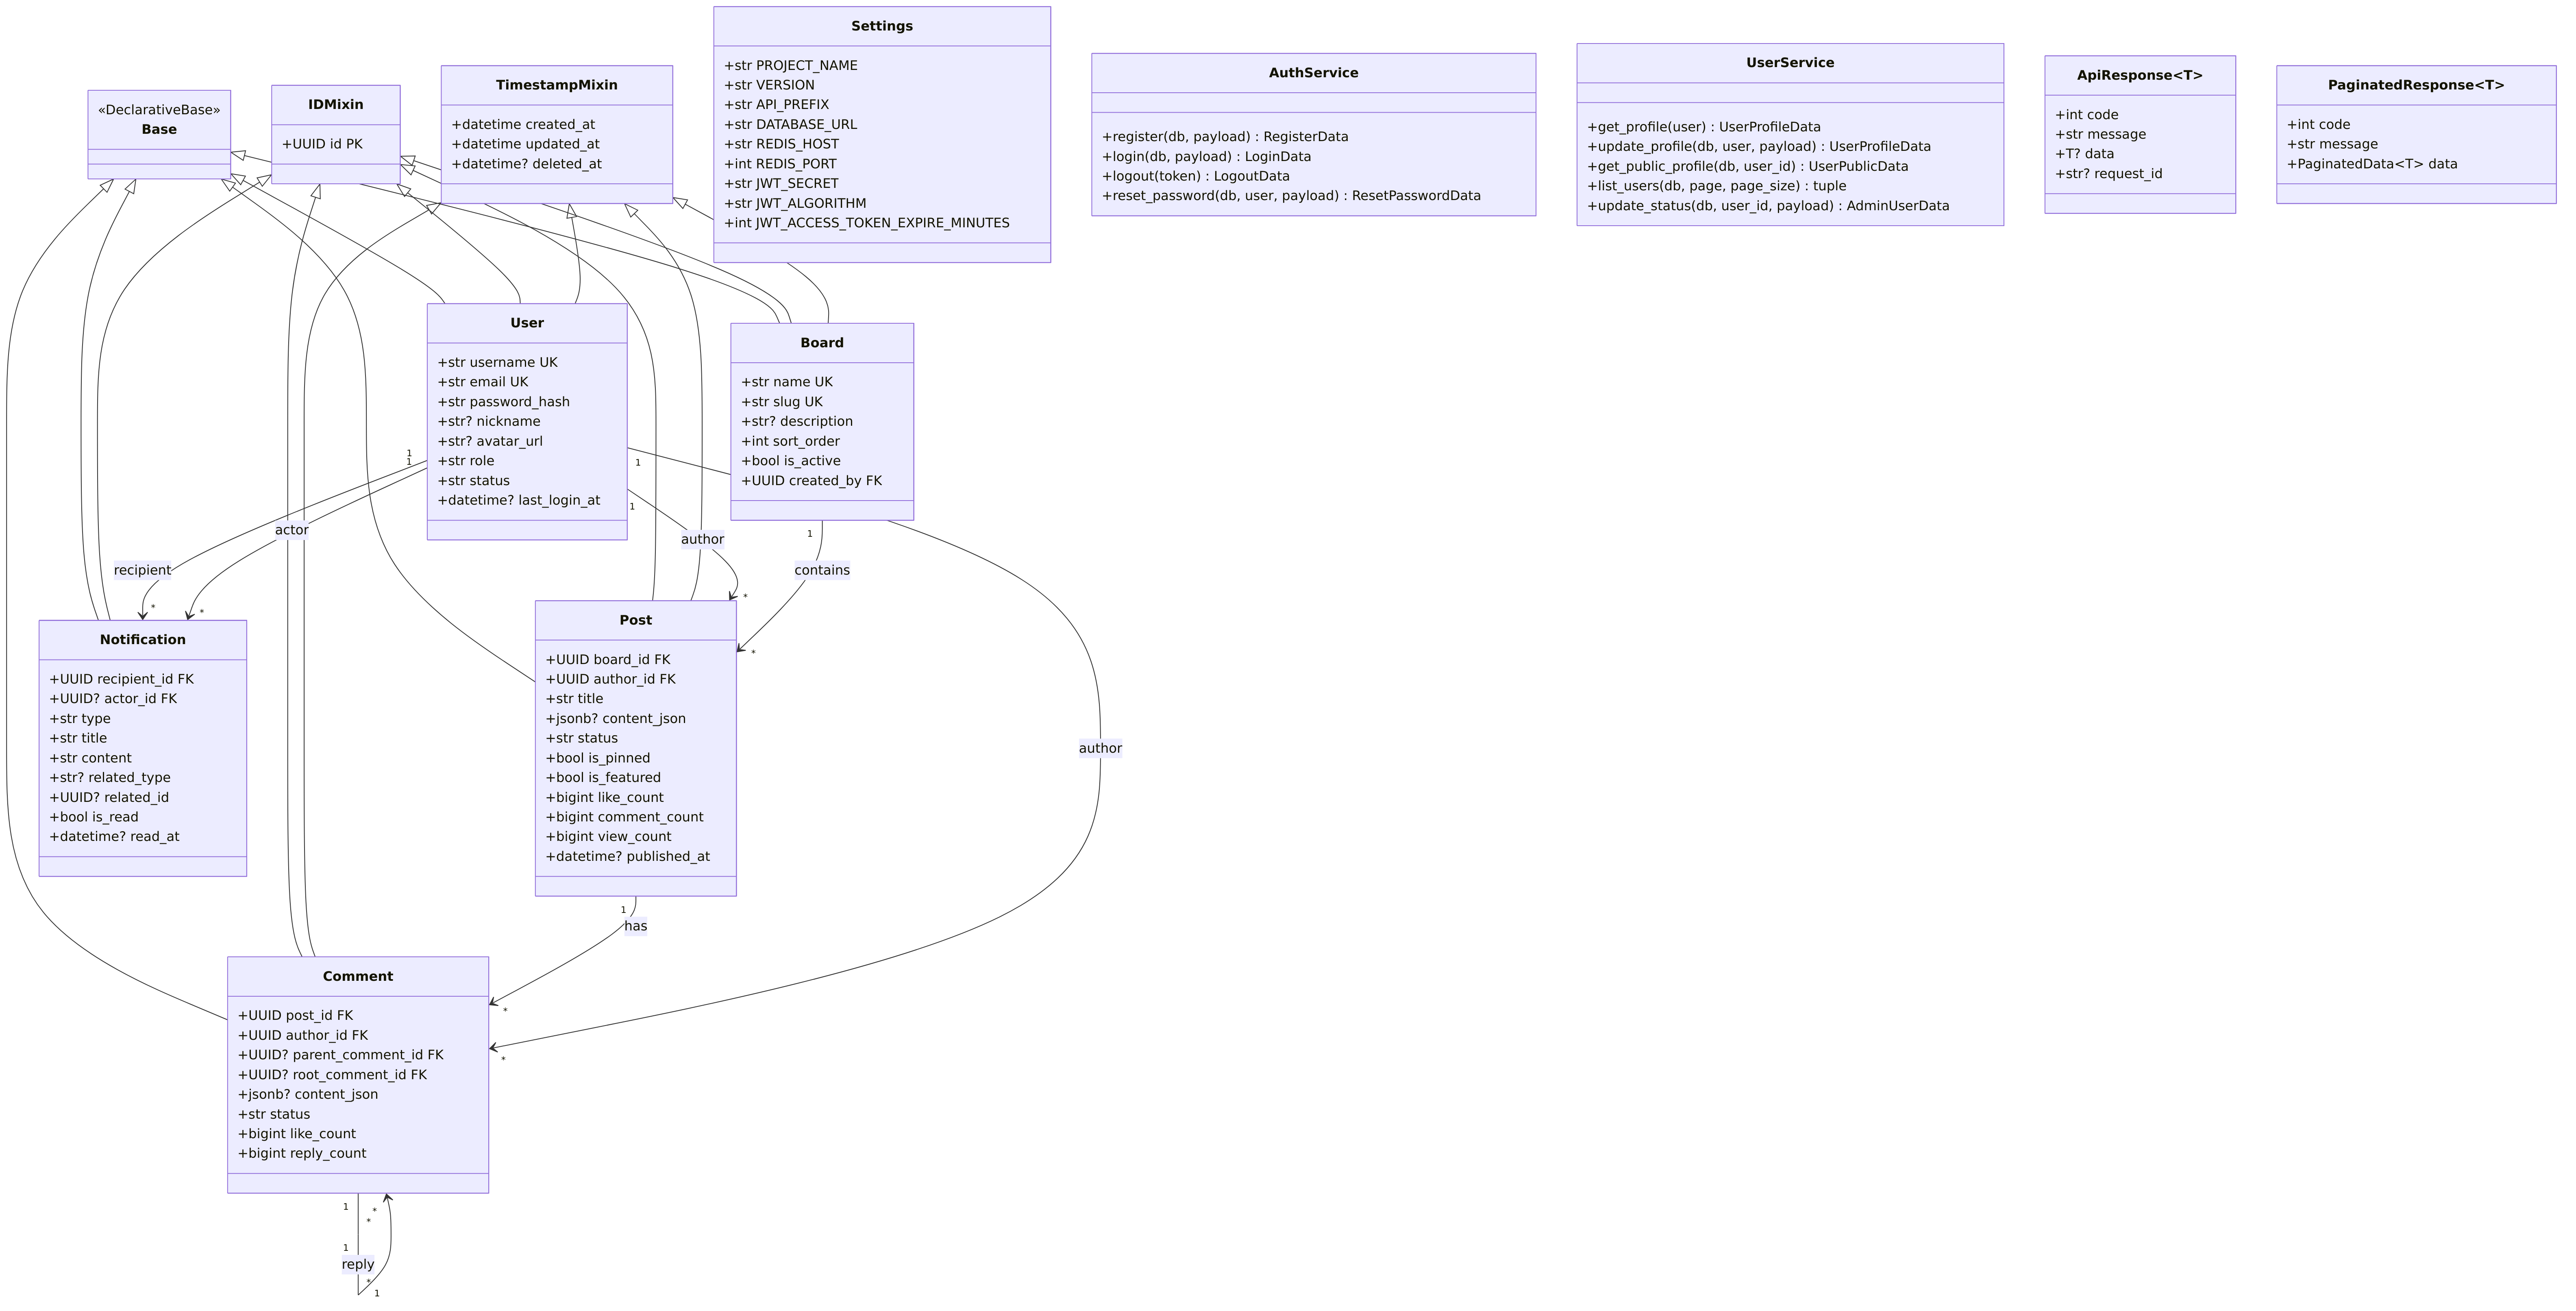
\includegraphics[width=\linewidth,height=0.88\textheight,keepaspectratio]{images/class_diagram.png}
\end{frame}

\begin{frame}{CRC Cards —— 核心类（1/2）}
    \small
    \centering
    \begin{tabular}{|p{4.8cm}|p{4.8cm}|}
        \hline
        \multicolumn{2}{|c|}{\textbf{User}} \\
        \hline
        \textbf{Responsibilities} & \textbf{Collaborators} \\
        \hline
        维护用户基本信息（用户名、邮箱、密码哈希） & AuthService \\
        记录角色（user/admin）与状态（active/banned） & Post, Comment \\
        维护最后登录时间 & Notification \\
        \hline
    \end{tabular}
    \vspace{0.3cm}

    \begin{tabular}{|p{4.8cm}|p{4.8cm}|}
        \hline
        \multicolumn{2}{|c|}{\textbf{Post}} \\
        \hline
        \textbf{Responsibilities} & \textbf{Collaborators} \\
        \hline
        存储帖子标题、内容、状态 & User（作者） \\
        维护置顶/加精标记 & Board（所属板块） \\
        聚合点赞数、评论数、浏览数 & Comment, PostLike \\
        \hline
    \end{tabular}
\end{frame}

\begin{frame}{CRC Cards —— 核心类（2/2）}
    \small
    \centering
    \begin{tabular}{|p{4.8cm}|p{4.8cm}|}
        \hline
        \multicolumn{2}{|c|}{\textbf{Comment}} \\
        \hline
        \textbf{Responsibilities} & \textbf{Collaborators} \\
        \hline
        存储评论内容、状态 & User（作者）, Post \\
        支持楼中楼回复（parent/root） & Comment（自身） \\
        聚合点赞数、回复数 & CommentLike \\
        \hline
    \end{tabular}
    \vspace{0.3cm}

    \begin{tabular}{|p{4.8cm}|p{4.8cm}|}
        \hline
        \multicolumn{2}{|c|}{\textbf{Notification}} \\
        \hline
        \textbf{Responsibilities} & \textbf{Collaborators} \\
        \hline
        记录通知类型（comment/reply/like/system） & User（接收人/触发人） \\
        维护已读状态与已读时间 & Post, Comment（关联对象） \\
        \hline
    \end{tabular}

    \vspace{0.3cm}

    \begin{tabular}{|p{4.8cm}|p{4.8cm}|}
        \hline
        \multicolumn{2}{|c|}{\textbf{Board}} \\
        \hline
        \textbf{Responsibilities} & \textbf{Collaborators} \\
        \hline
        存储板块名称、slug、描述、排序值 & User（创建人） \\
        维护板块启用状态（is\_active） & Post（所含帖子） \\
        支持按 sort\_order 排序展示 & AdminPanel（管理操作） \\
        \hline
    \end{tabular}
\end{frame}

\begin{frame}{CRC Cards —— 服务层}
    \small
    \centering
    \begin{tabular}{|p{4.8cm}|p{4.8cm}|}
        \hline
        \multicolumn{2}{|c|}{\textbf{AuthService}} \\
        \hline
        \textbf{Responsibilities} & \textbf{Collaborators} \\
        \hline
        用户注册（校验唯一性、密码哈希） & User, security.py \\
        用户登录（校验密码、生成 JWT） & User, Redis（Token 黑名单） \\
        用户登出（Token 加入黑名单） & Redis \\
        密码重置（校验旧密码、更新哈希） & User, security.py \\
        \hline
    \end{tabular}
    \vspace{0.3cm}

    \begin{tabular}{|p{4.8cm}|p{4.8cm}|}
        \hline
        \multicolumn{2}{|c|}{\textbf{UserService}} \\
        \hline
        \textbf{Responsibilities} & \textbf{Collaborators} \\
        \hline
        获取/更新当前用户资料 & User \\
        获取用户公开资料 & User \\
        管理员：用户列表分页查询 & User \\
        管理员：更新用户状态（封禁/解封/角色） & User, Notification \\
        \hline
    \end{tabular}
\end{frame}

\begin{frame}{安全性分析}
    \begin{columns}
        \column{0.48\textwidth}
        \begin{block}{认证与授权安全}
            \begin{itemize}
                \item 密码使用 Argon2 哈希存储（pwdlib）
                \item JWT Token（HS256）设有效期，支持黑名单登出
                \item 接口级 RBAC 权限控制（user/admin）
            \end{itemize}
        \end{block}
        \column{0.48\textwidth}
        \begin{block}{数据与传输安全}
            \begin{itemize}
                \item 核心业务数据软删除（deleted\_at），可恢复
                \item SQLAlchemy ORM 防 SQL 注入
                \item 预留 HTTPS 传输加密部署方案
            \end{itemize}
        \end{block}
    \end{columns}
    \vspace{0.3cm}
    \begin{columns}
        \column{0.48\textwidth}
        \begin{block}{接口安全}
            \begin{itemize}
                \item 登录/注册接口速率限制（slowapi），防暴力破解
                \item 输入参数 Pydantic 校验，防畸形数据
            \end{itemize}
        \end{block}
        \column{0.48\textwidth}
    \end{columns}
\end{frame}

\begin{frame}{性能需求}
    \begin{columns}
        \column{0.48\textwidth}
        \begin{block}{响应时间指标}
            \begin{itemize}
                \item 帖子列表接口响应时间 $<$ 200ms
                \item 数据库单表分页查询 $<$ 100ms
                \item 登录/注册接口 $<$ 300ms
            \end{itemize}
        \end{block}
        \column{0.48\textwidth}
        \begin{block}{并发与容量}
            \begin{itemize}
                \item 支持并发用户 500+（MVP 阶段）
                \item 图片/附件预留对象存储接口
                \item Redis 缓存热点数据（Token、计数）
            \end{itemize}
        \end{block}
    \end{columns}
    \vspace{0.3cm}
    \begin{columns}
        \column{0.48\textwidth}
        \begin{block}{数据库优化}
            \begin{itemize}
                \item 索引优化（created\_at、board\_id、user\_id）
                \item 分页查询避免深页性能衰减
                \item 计数字段冗余，减少实时聚合
            \end{itemize}
        \end{block}
        \column{0.48\textwidth}
        \begin{block}{可用性目标}
            \begin{itemize}
                \item 系统可用性目标 \textit{99.9\%}
                \item 核心业务数据软删除，可恢复
                \item 健康检查端点（/health）用于监控
            \end{itemize}
        \end{block}
    \end{columns}
\end{frame}

\begin{frame}{UI 设计 —— 页面流程图}
    \centering
    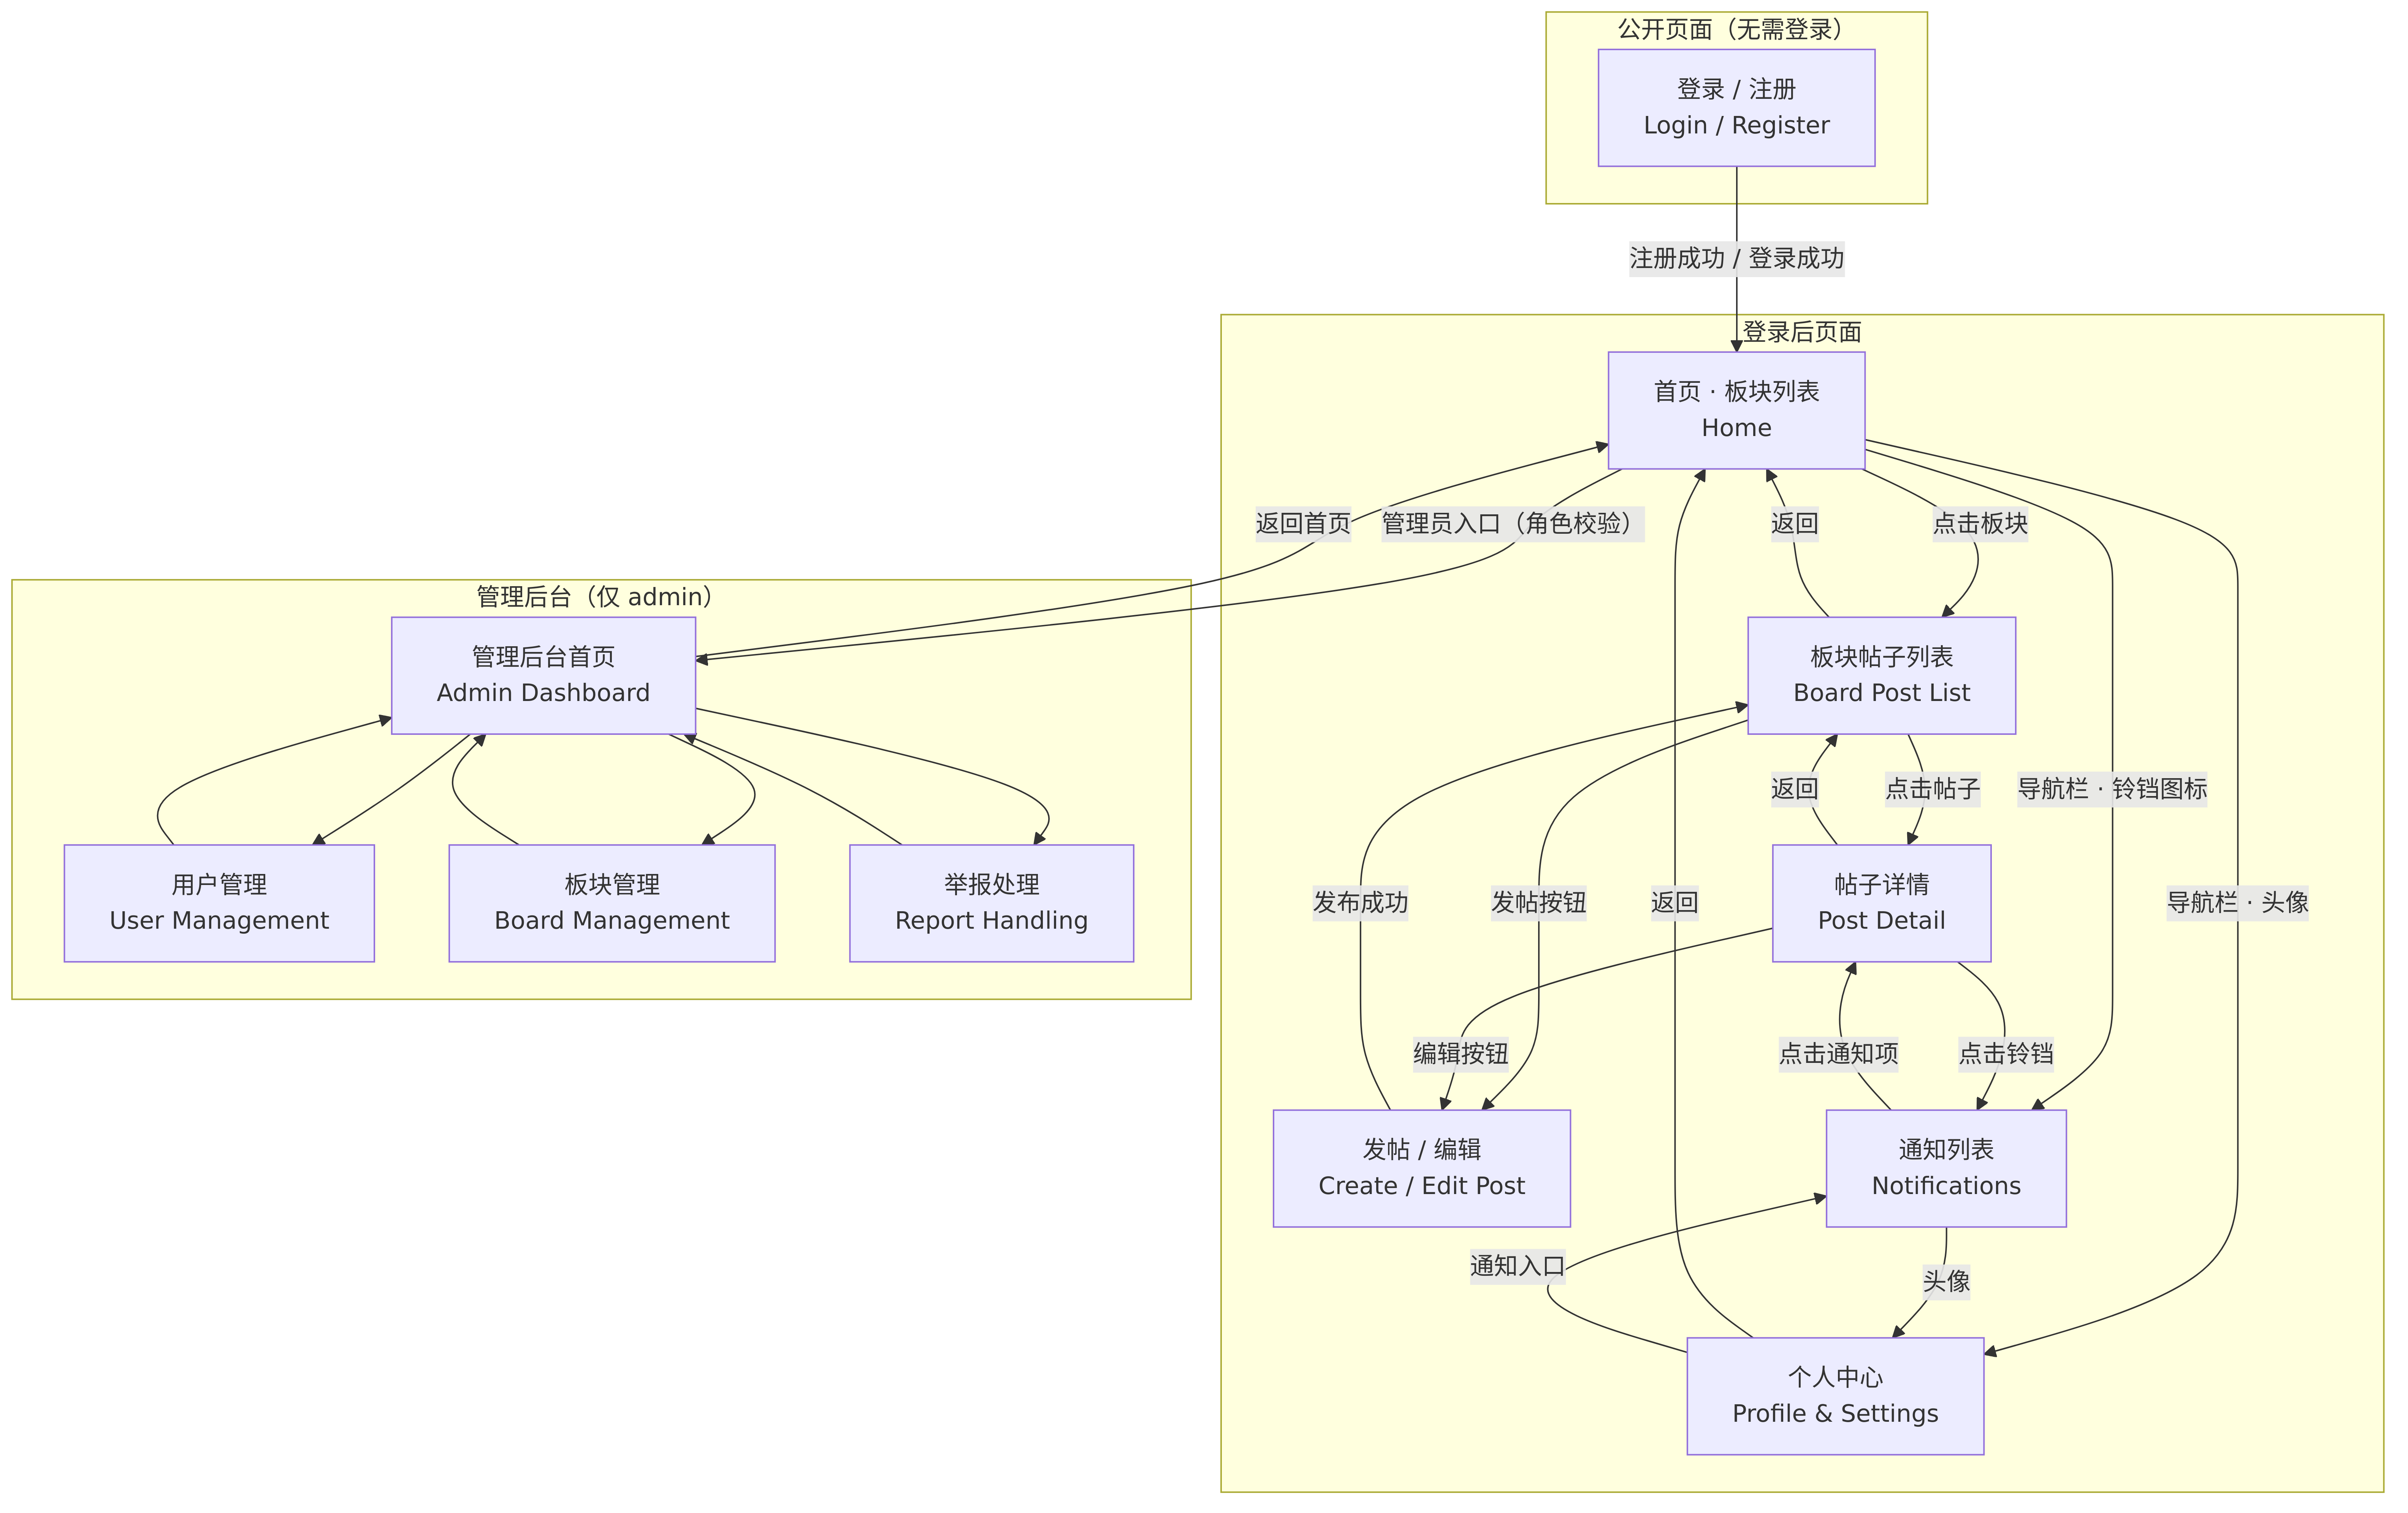
\includegraphics[width=\linewidth,height=0.88\textheight,keepaspectratio]{images/page_flow.png}
\end{frame}

\begin{frame}{UI 设计 —— 核心页面线框图（1/3）}
    \centering
    \begin{columns}
        \column{0.32\textwidth}
        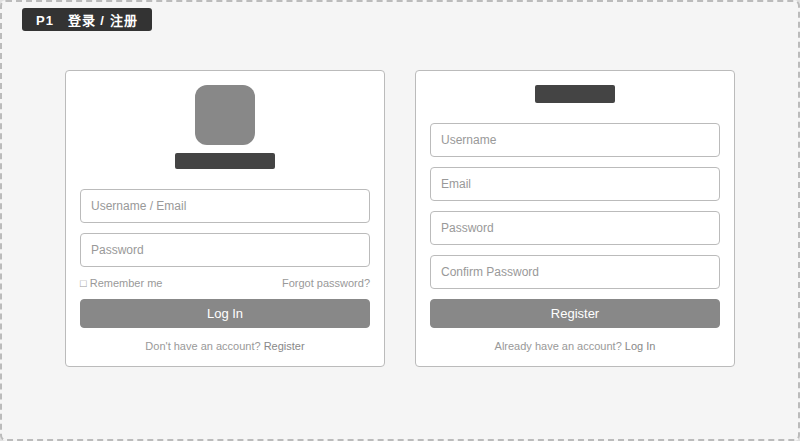
\includegraphics[width=\linewidth,height=0.38\textheight,keepaspectratio]{images/wireframe_P1_登录_注册.png}
        \vspace{0.02\textheight}
        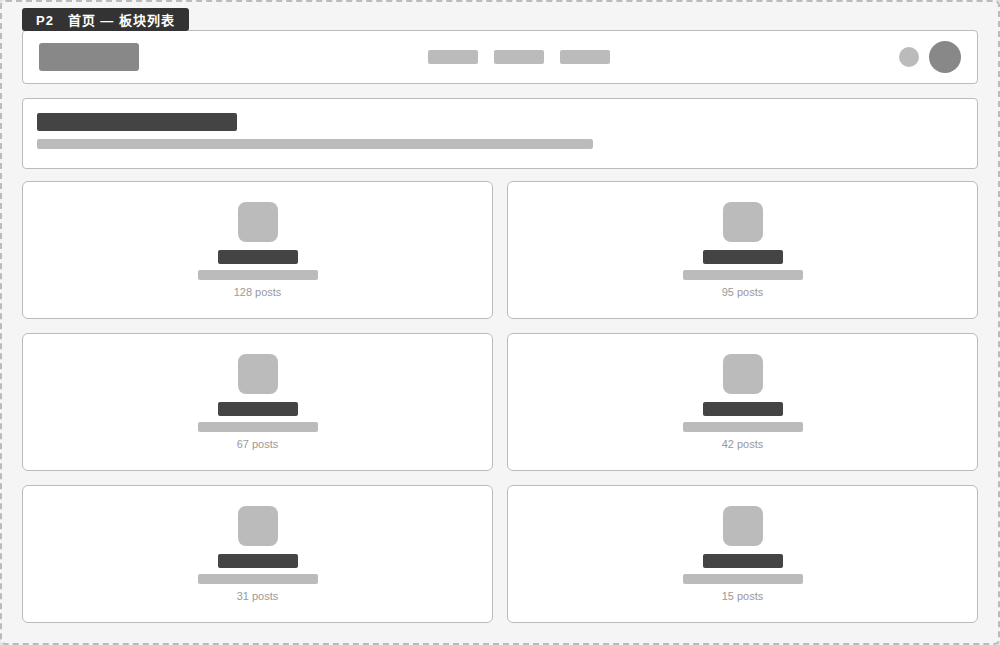
\includegraphics[width=\linewidth,height=0.38\textheight,keepaspectratio]{images/wireframe_P2_首页_板块列表.png}
        \column{0.32\textwidth}
        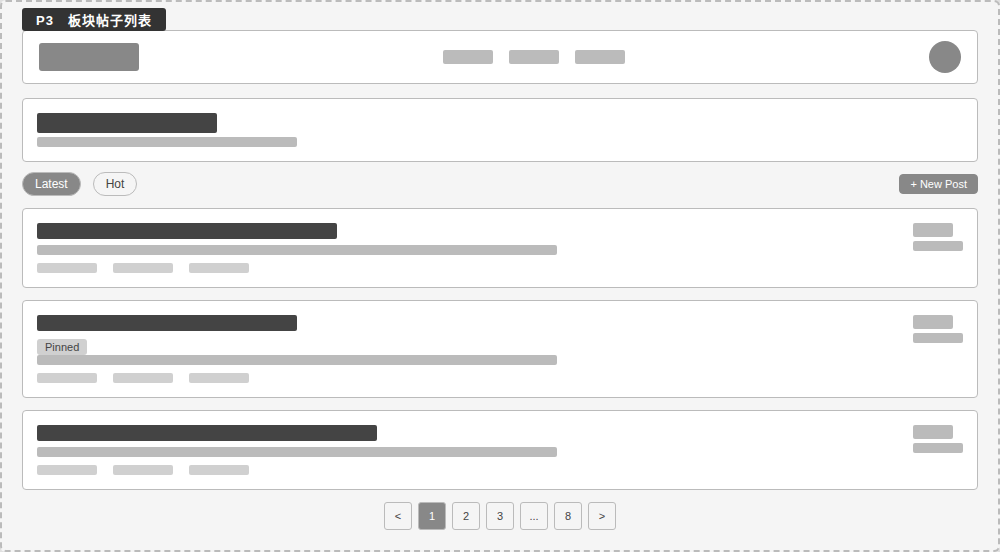
\includegraphics[width=\linewidth,height=0.80\textheight,keepaspectratio]{images/wireframe_P3_板块帖子列表.png}
        \column{0.32\textwidth}
        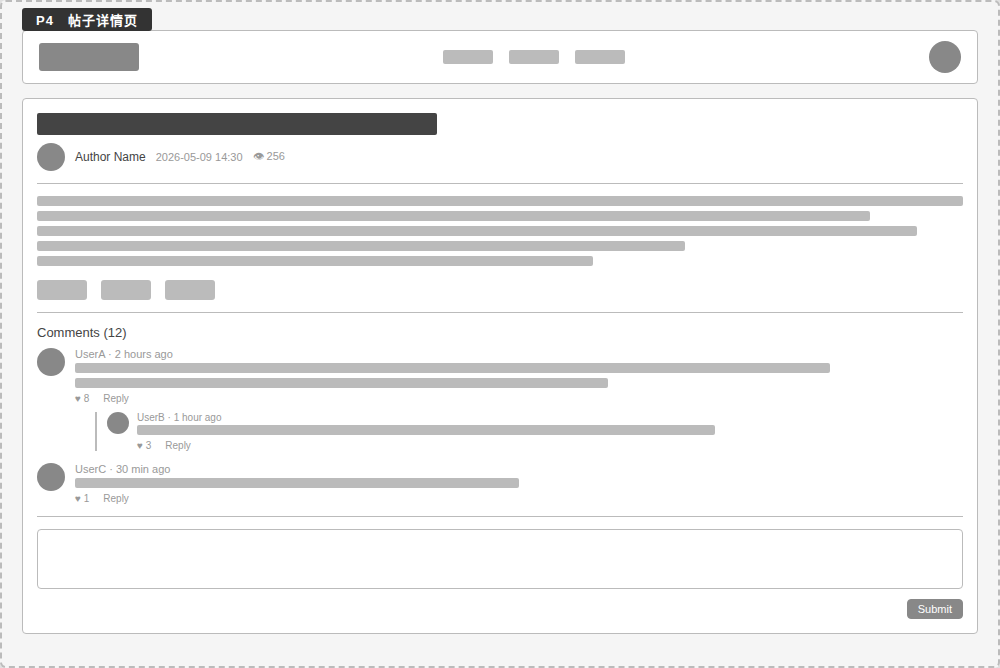
\includegraphics[width=\linewidth,height=0.80\textheight,keepaspectratio]{images/wireframe_P4_帖子详情页.png}
    \end{columns}
\end{frame}

\begin{frame}{UI 设计 —— 核心页面线框图（2/3）}
    \centering
    \begin{columns}
        \column{0.48\textwidth}
        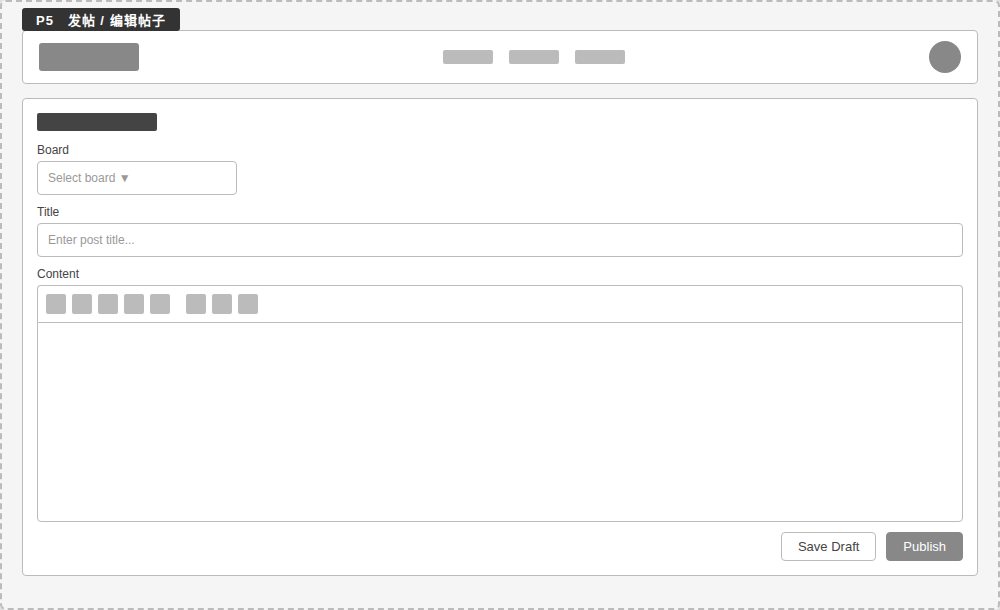
\includegraphics[width=\linewidth,height=0.88\textheight,keepaspectratio]{images/wireframe_P5_发帖_编辑帖子.png}
        \column{0.48\textwidth}
        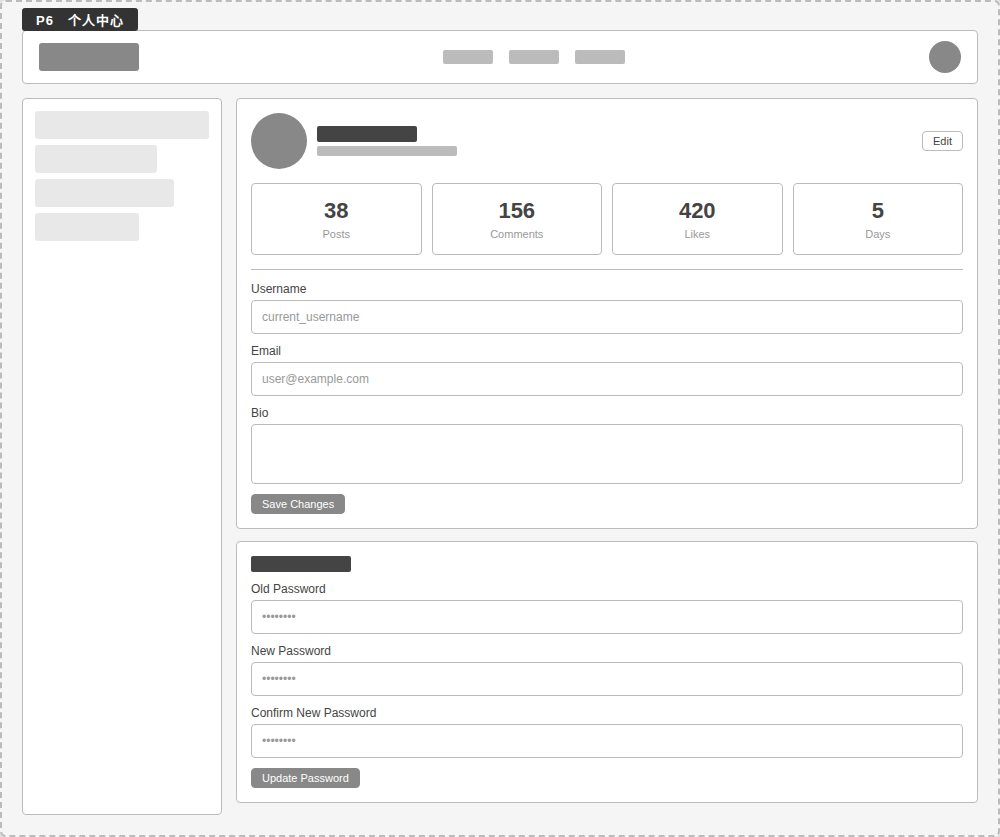
\includegraphics[width=\linewidth,height=0.88\textheight,keepaspectratio]{images/wireframe_P6_个人中心.png}
    \end{columns}
\end{frame}

\begin{frame}{UI 设计 —— 核心页面线框图（3/3）}
    \centering
    \begin{columns}
        \column{0.32\textwidth}
        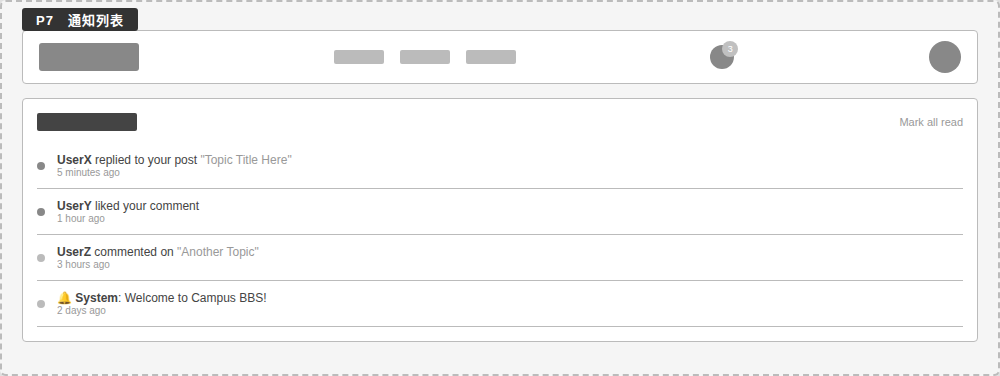
\includegraphics[width=\linewidth,height=0.88\textheight,keepaspectratio]{images/wireframe_P7_通知列表.png}
        \column{0.32\textwidth}
        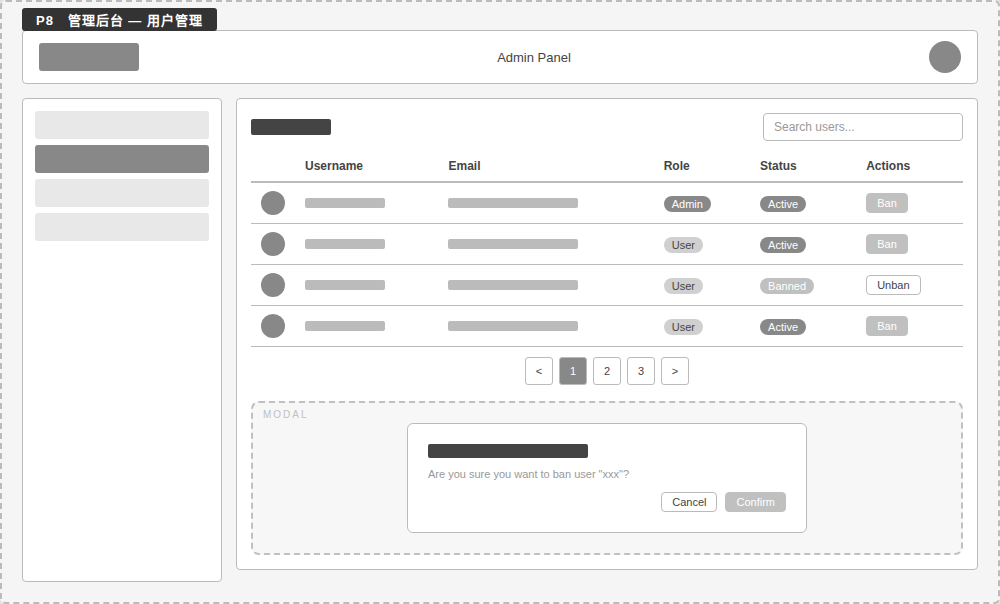
\includegraphics[width=\linewidth,height=0.88\textheight,keepaspectratio]{images/wireframe_P8_管理后台_用户管理.png}
        \column{0.32\textwidth}
        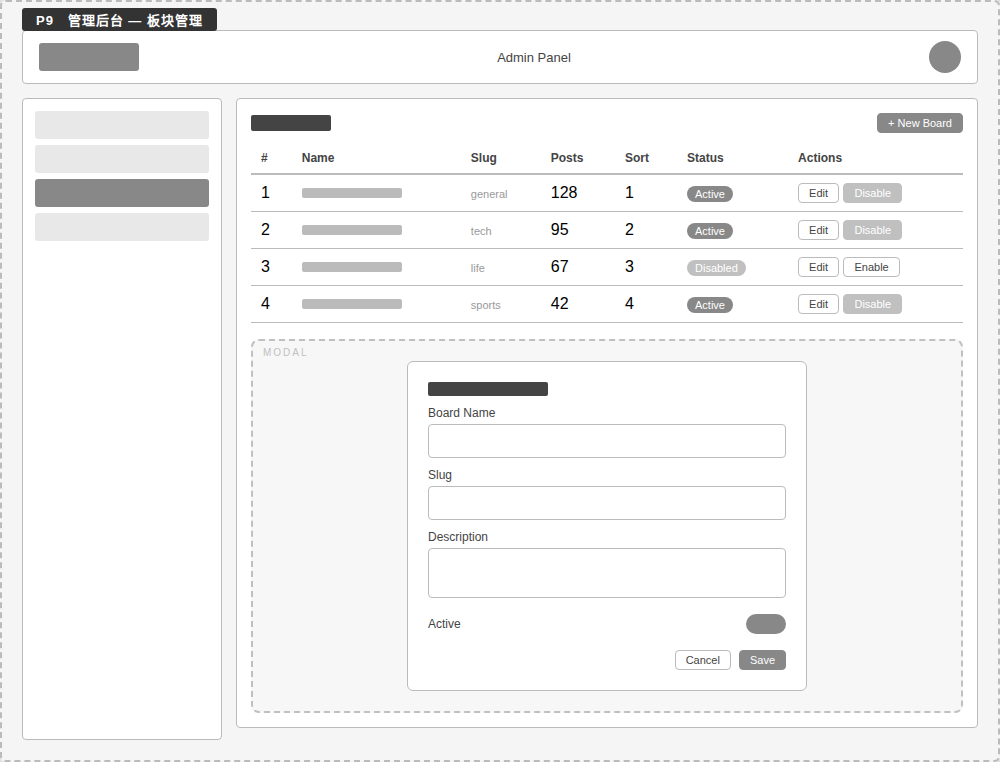
\includegraphics[width=\linewidth,height=0.88\textheight,keepaspectratio]{images/wireframe_P9_管理后台_板块管理.png}
    \end{columns}
\end{frame}

% ============================================================
\section{项目计划}
% ============================================================

\begin{frame}{文档质量}
    \begin{columns}
        \column{0.48\textwidth}
        \begin{block}{文档体系}
            \begin{itemize}
                \item \textbf{DesignDiagrams.md}：UML 类图、用例图、状态图等
                \item \textbf{DatabaseDesign.md}：数据库表结构设计与 ER 图
                \item \textbf{DevelopmentSpecification.md}：代码规范、API 设计规范
                \item \textbf{ProjectRequirements.md}：功能性与非功能性需求
            \end{itemize}
        \end{block}
        \column{0.48\textwidth}
        \begin{block}{质量保障措施}
            \begin{itemize}
                \item API 文档采用 FastAPI 自动生成的交互式文档
                \item 文档随迭代同步更新，版本控制入 Git
                \item 代码提交前通过 black + ruff 自动格式化
                \item PR 必须经过代码审查与文档核对
            \end{itemize}
        \end{block}
    \end{columns}
\end{frame}

\begin{frame}{项目范围}
    \begin{columns}
        \column{0.48\textwidth}
        \begin{block}{MVP 必做范围}
            \begin{enumerate}
                \item 用户与认证子系统（Part1）
                \item 帖子与分区子系统（Part2）
                \item 评论与互动子系统（Part3）
                \item 通知基础子系统（Part4 基础）
                \item 管理后台基础（Part6 基础）
            \end{enumerate}
        \end{block}
        \column{0.48\textwidth}
        \begin{block}{迭代扩展范围}
            \begin{itemize}
                \item \textbf{迭代一}：系统公告与站内信；公告管理、举报处理
                \item \textbf{迭代二}：关键词搜索、热门排序
                \item \textbf{迭代三}：个性化推荐；操作审计与日志
            \end{itemize}
        \end{block}
    \end{columns}
    \vspace{0.3cm}
    \begin{block}{范围约束}
        \begin{itemize}
            \item 不实现即时聊天（IM）；不实现第三方支付；图片/附件仅预留接口，MVP 阶段不接入真实对象存储
        \end{itemize}
    \end{block}
\end{frame}

\begin{frame}{Process Model —— 开发过程模型}
    \begin{block}{迭代式开发模型（Iterative Model）}
        \begin{itemize}
            \item 采用短周期迭代，每个迭代 1 周，产出可演示的增量版本。
            \item MVP 阶段聚焦核心闭环（注册 $\rightarrow$ 发帖 $\rightarrow$ 评论 $\rightarrow$ 通知）。
            \item 每轮迭代结束进行小组 Review 与需求微调。
        \end{itemize}
    \end{block}
    \pause
    \begin{block}{敏捷实践}
        \begin{itemize}
            \item Git 分支管理：feature $\rightarrow$ develop $\rightarrow$ main，PR 代码审查。
            \item 持续集成：Husky pre-commit（black + ruff），pytest 自动测试。
            \item 文档驱动：API 文档与数据库设计文档随迭代同步更新。
        \end{itemize}
    \end{block}
\end{frame}

\begin{frame}{Scale Estimation —— 规模估算}
    \begin{columns}
        \column{0.5\textwidth}
        \begin{block}{功能点估算}
            \begin{itemize}
                \item 用户认证模块：\textasciitilde 8 FP
                \item 帖子/分区模块：\textasciitilde 10 FP
                \item 评论/互动模块：\textasciitilde 8 FP
                \item 通知模块：\textasciitilde 6 FP
                \item 管理后台：\textasciitilde 8 FP
                \item 搜索推荐（迭代）：\textasciitilde 6 FP
            \end{itemize}
        \end{block}
        \column{0.5\textwidth}
        \begin{block}{代码规模估算}
            \begin{itemize}
                \item 后端（Python）：\textasciitilde 4,000--5,000 LOC
                \item 前端（TS）：\textasciitilde 6,000--8,000 LOC
                \item 测试代码：\textasciitilde 1,500--2,000 LOC
                \item 文档/配置：\textasciitilde 2,000 LOC
            \end{itemize}
        \end{block}
    \end{columns}
    \vspace{0.3cm}
    \begin{block}{工期估算}
        \begin{itemize}
            \item 总工期约 6 周（MVP 3 周 + 迭代一 1 周 + 迭代二 1 周 + 迭代三 1 周缓冲）。
            \item 团队规模 6 人，总工作量约 216 人时（按每人每周 6 小时投入估算）。
        \end{itemize}
    \end{block}
\end{frame}

\begin{frame}{资源配置}
    \begin{columns}
        \column{0.48\textwidth}
        \begin{block}{人力资源}
            \begin{itemize}
                \item 组长 1 人：架构设计、代码审核、Git 管理
                \item 前端 2 人：用户端 / 管理端界面开发
                \item 后端 2 人：业务接口与数据库开发
                \item 测试兼文档 1 人：测试用例、CI/CD、文档维护
            \end{itemize}
        \end{block}
        \column{0.48\textwidth}
        \begin{block}{软硬件环境}
            \begin{itemize}
                \item 开发环境：Python 3.14 + FastAPI + PostgreSQL + Redis
                \item 前端：Vue + TypeScript + pnpm
                \item 容器化：Docker Compose 一键启动依赖服务
                \item 版本控制：Git + Husky hooks（lint-staged）
            \end{itemize}
        \end{block}
    \end{columns}
    \vspace{0.3cm}
    \begin{block}{工具链}
        \begin{itemize}
            \item 格式化：black；代码检查：ruff；测试：pytest；包管理：uv（后端）/ pnpm（前端）
        \end{itemize}
    \end{block}
\end{frame}

\begin{frame}{交付物定义}
    \small
    \centering
    \begin{tabular}{clp{6cm}}
        \toprule
        \textbf{阶段} & \textbf{交付物} & \textbf{说明} \\
        \midrule
        MVP & 源代码 & 后端核心接口 + 前端基础页面 \\
        MVP & 数据库迁移脚本 & Alembic 迁移文件 \\
        MVP & API 文档 & FastAPI 自动生成交互式文档 \\
        \midrule
        迭代一 & 管理后台 & 用户/板块/公告管理功能 \\
        迭代一 & 通知系统 & 站内信与系统公告 \\
        \midrule
        迭代二 & 搜索功能 & 关键词搜索与热门排序 \\
        \midrule
        迭代三 & 推荐模块 & 个性化推荐（可选） \\
        迭代三 & 审计日志 & 操作审计与日志查询 \\
        \midrule
        结项 & 设计文档 & UML 图、数据库设计、需求文档 \\
        结项 & 测试报告 & 单元测试、集成测试报告 \\
        \bottomrule
    \end{tabular}
\end{frame}

\begin{frame}{任务与计划 —— 功能优先级与迭代规划}
    \small
    \centering
    \begin{tabular}{clp{6cm}}
        \toprule
        \textbf{优先级} & \textbf{子系统} & \textbf{说明} \\
        \midrule
        MVP 必做 & Part1、Part2、Part3 & 用户认证、帖子分区、评论互动 \\
        MVP 必做 & Part4（基础） & 评论/回复/点赞通知、未读计数 \\
        MVP 必做 & Part6（基础） & 用户管理、板块管理 \\
        \midrule
        迭代一 & Part4（完整） & 系统公告与站内信 \\
        迭代一 & Part6（完整） & 公告管理、举报处理 \\
        \midrule
        迭代二 & Part5 & 关键词搜索、热门排序 \\
        \midrule
        迭代三 & Part5（进阶） & 个性化推荐 \\
        迭代三 & Part6（进阶） & 操作审计与日志 \\
        \bottomrule
    \end{tabular}
\end{frame}

\begin{frame}{任务与计划 —— 功能迭代路线图}
    \centering
    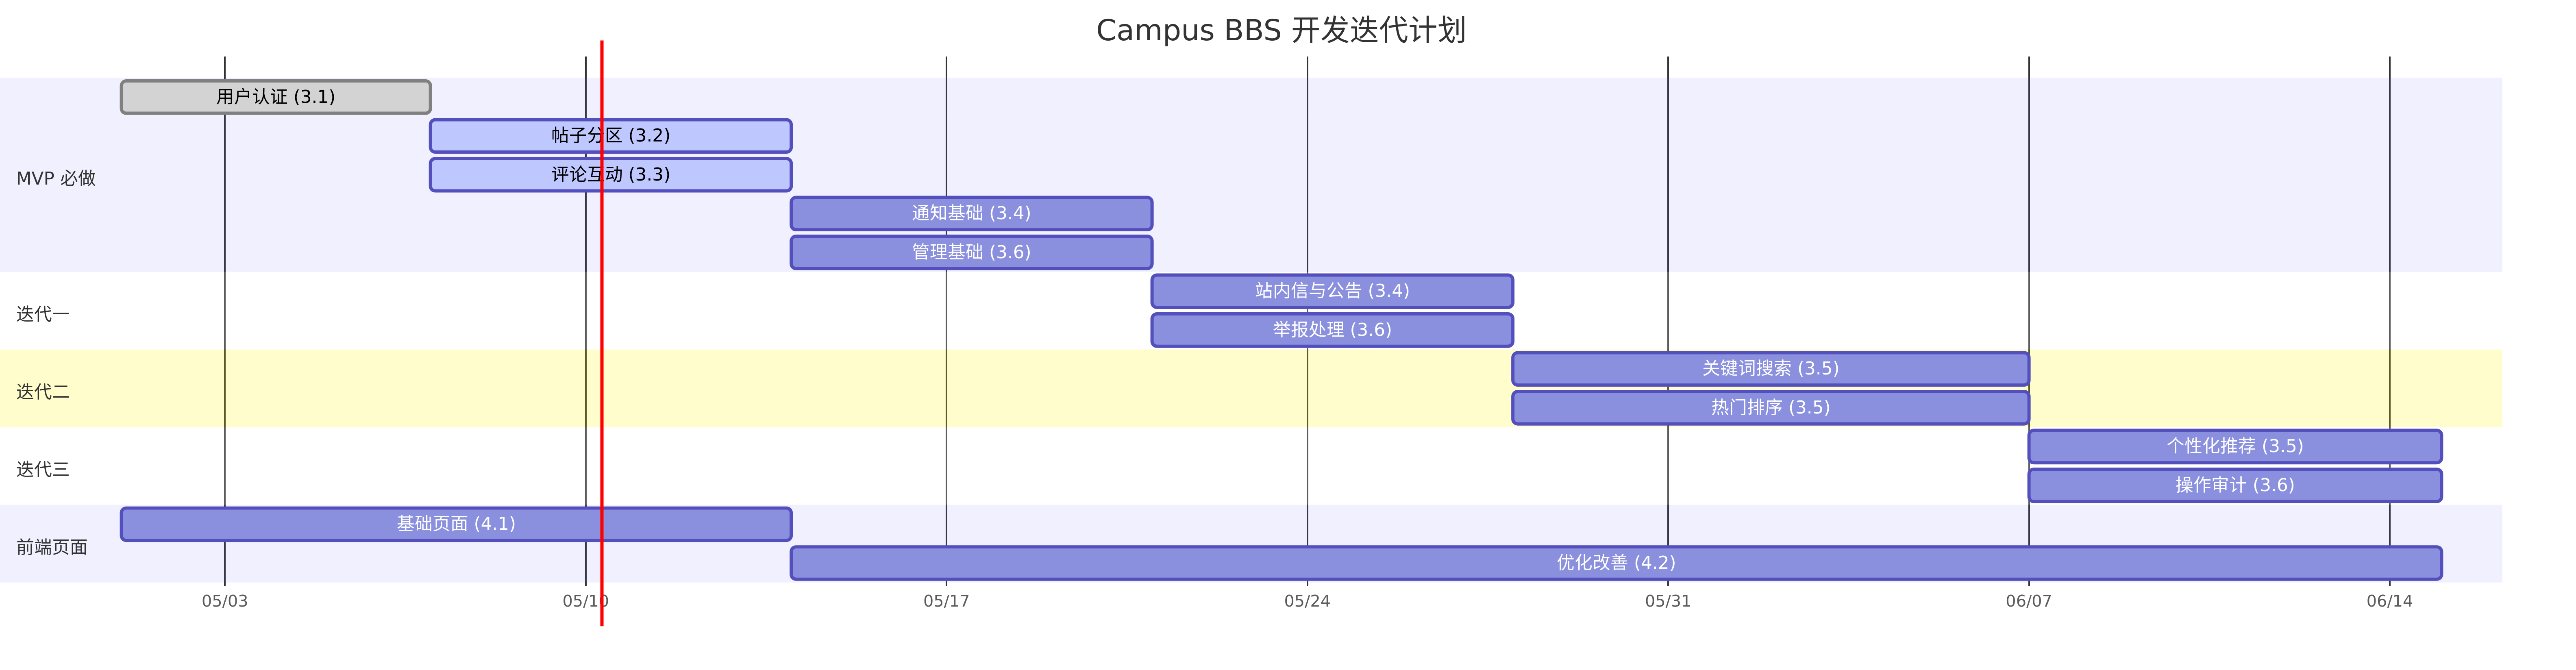
\includegraphics[width=\linewidth,height=0.88\textheight,keepaspectratio]{images/gantt.png}
\end{frame}

\begin{frame}{风险分析}
    \small
    \centering
    \begin{tabular}{p{3.2cm}ccp{4.5cm}}
        \toprule
        \textbf{风险项} & \textbf{概率} & \textbf{影响} & \textbf{应对措施} \\
        \midrule
        组员时间冲突 & 中 & 高 & Issue 驱动，组员承接任务，灵活安排时间 \\
        数据库性能瓶颈 & 低 & 中 & 索引优化 + 分页 + 预留 Redis 缓存扩展 \\
        需求变更 & 中 & 中 & 迭代规划预留 20\% 缓冲时间，优先保障 MVP \\
        \bottomrule
    \end{tabular}
\end{frame}

\begin{frame}{文档质量保障}
    \begin{columns}
        \column{0.48\textwidth}
        \begin{block}{代码文档}
            \begin{itemize}
                \item 接口文档：FastAPI 自动生成，随代码同步更新
                \item 核心函数添加 docstring，说明参数与返回值
                \item 复杂业务逻辑添加行内注释
            \end{itemize}
        \end{block}
        \column{0.48\textwidth}
        \begin{block}{设计文档}
            \begin{itemize}
                \item 需求变更必须同步更新 ProjectRequirements.md
                \item 数据库变更必须同步更新 DatabaseDesign.md 并生成迁移脚本
                \item UML 图使用 Mermaid 绘制，版本入 Git
            \end{itemize}
        \end{block}
    \end{columns}
    \vspace{0.3cm}
    \begin{block}{质量检查清单}
        \begin{itemize}
            \item PR 合并前：代码审查通过、测试通过、文档已更新、black + ruff 检查通过
        \end{itemize}
    \end{block}
\end{frame}

\begin{frame}{总结与下一步}
    \begin{block}{当前进展}
        \begin{itemize}
            \item 用户与认证子系统（Part1）已实现
            \item 帖子分区（Part2）、评论互动（Part3）、通知（Part4）、管理后台（Part6）路由已定义
            \item 前端页面线框图设计完成
            \item 数据库迁移与基础架构搭建完成
        \end{itemize}
    \end{block}
    \pause
    \begin{block}{下一步计划}
        \begin{itemize}
            \item 完成 MVP 阶段各子系统的核心接口实现
            \item 推进前端页面开发与管理端界面
            \item 编写测试用例，配置 CI/CD 流程
        \end{itemize}
    \end{block}
\end{frame}

\begin{frame}
    \centering
    \Huge 感谢聆听！
    \vspace{1cm}

    \normalsize
    \textit{Q \& A}
\end{frame}

\end{document}
